% --- Document Class ---
\documentclass[12pt,a4paper]{report}

% --- Font Encoding (required for accented characters: ü, ş, etc.) ---
\usepackage[T1]{fontenc}
\usepackage[utf8]{inputenc}   % declare UTF-8 source encoding so listings handles section symbol, em dash, ellipsis correctly

% --- Times Text Font (pdflatex compatible) ---
\usepackage{newtxtext,newtxmath}

% --- Page Geometry ---
\usepackage[a4paper, top=2.5cm, bottom=2.5cm, left=3cm, right=2.5cm, headheight=15pt]{geometry}

% --- float package: lets a table/figure be pinned with [H] so it never
%     gets bumped onto its own "float page". Isolated float pages get
%     vertically centered by LaTeX with large rubber space above/below,
%     which is what made Table 3.1 look like it filled a whole page. ---
\usepackage{float}

% --- Text Positioning for Cover Page ---
\usepackage[absolute]{textpos}
\usepackage{graphicx}
\setlength{\TPHorizModule}{1pt}
\setlength{\TPVertModule}{1pt}
\textblockorigin{0pt}{0pt}

% --- Line Spacing (Single line as per VGU requirement) ---
\usepackage{setspace}
\singlespacing

% --- Page Numbering & Headers/Footers ---
\usepackage{seqsplit}
\usepackage{fancyhdr}
\pagestyle{fancy}
\fancyhf{}
\fancyhead[L]{\nouppercase{\leftmark}}
\fancyfoot[C]{\thepage}
\renewcommand{\headrulewidth}{0.4pt}
\renewcommand{\chaptermark}[1]{\markboth{\chaptername\ \thechapter.\ #1}{}}
\fancypagestyle{plain}{%
  \fancyhf{}%
  \fancyfoot[C]{\thepage}%
  \renewcommand{\headrulewidth}{0pt}%
}
\fancypagestyle{preliminary}{%
  \fancyhf{}%
  \fancyfoot[C]{\thepage}%
  \renewcommand{\headrulewidth}{0pt}%
}
\fancypagestyle{empty}{%
  \fancyhf{}%
  \renewcommand{\headrulewidth}{0pt}%
}

% --- Table of Contents ---
\usepackage[nottoc,notlof,notlot]{tocbibind}

% --- Chapter Heading Style (compact "N.  Title" format, matching VGU reference) ---
\usepackage{titlesec}
\titleformat{\chapter}[hang]
  {\normalfont\Large\bfseries}{\thechapter.}{10pt}{\Large\bfseries}
\titlespacing*{\chapter}{0pt}{0pt}{20pt}
% Keep the same compact style for unnumbered chapters (Declaration, Abstract, Bibliography, etc.)
\titleformat{name=\chapter,numberless}[hang]
  {\normalfont\Large\bfseries}{}{0pt}{\Large\bfseries}
\titlespacing*{name=\chapter,numberless}{0pt}{0pt}{20pt}

% --- TikZ for org chart ---
\usepackage{tikz}
\usetikzlibrary{positioning, shapes.geometric, fit, calc}
\usepackage{pgfplots}
\pgfplotsset{compat=1.18}

% Externalize disabled - not well supported on Overleaf
% \usepgfplotslibrary{external}
% \tikzexternalize
% \tikzset{external/system call={pdflatex -interaction=batchmode -halt-on-error -shell-escape #1}}

% --- Tables ---
\usepackage{booktabs}
\usepackage{array}
\usepackage[table]{xcolor}
\usepackage{longtable}

% --- Directory-tree diagrams (Figure 5.1) ---
\usepackage{forest}

% --- Code listings ---
\usepackage{listings}
\usepackage{caption}
\usepackage{amsmath}
\usepackage[backend=biber, style=apa, sorting=none, uniquelist=false]{biblatex}
\DeclareLanguageMapping{english}{english-apa}
% APA 7 numbered reference list: labels are [1], [2], ... by citation order.
% The bibliography environment is overridden to print labelnumber at the start
% of each entry (the default apa.bbx environment does not print it).
\ExecuteBibliographyOptions{labelnumber}
\DeclareFieldFormat{labelnumberwidth}{\mkbibbrackets{#1}}
\makeatletter
\defbibenvironment{bibliography}%
  {\list{\printtext[labelnumberwidth]{\printfield{labelprefix}\printfield{labelnumber}}}%
     {\setlength{\labelwidth}{\labelnumberwidth}%
      \setlength{\leftmargin}{\labelwidth}%
      \setlength{\labelsep}{\biblabelsep}%
      \addtolength{\leftmargin}{\labelsep}%
      \setlength{\itemsep}{1\baselineskip}%
      \setlength{\parsep}{\bibparsep}}}%
  {\endlist}%
  {\item}
\makeatother
\addbibresource{references.bib}
% Override APA 7 sentence-case conversion: keep title case as written in .bib
\DeclareFieldFormat{apacase}{#1}
\DeclareFieldFormat{title}{#1\isdot}
\DeclareFieldFormat[article,inbook,incollection,periodical,misc,legislation,legadminmaterial,jurisdiction,inproceedings,legal]{title}{#1\isdot}
% Reference list uses biblatex-apa format with numbering labels [1], [2], ... in
% citation order. The \defbibenvironment override above is required because the
% default apa.bbx bibliography environment does not print the labelnumber field.

% Colors matching a syntax-highlighted editor theme
\definecolor{codebg}{gray}{0.97}
\definecolor{codeframe}{gray}{0.55}
\definecolor{codekeyword}{RGB}{0,0,190}
\definecolor{codecomment}{RGB}{0,128,0}
\definecolor{codestring}{RGB}{163,21,21}
\definecolor{codenumber}{gray}{0.5}

% --- TypeScript language definition for listings ---
% The `listings` package does not ship a built-in TypeScript definition on
% every TeX distribution/version (some local MiKTeX/TeX Live installs are
% missing it, producing "Couldn't load requested language" /
% "language typescript undefined"). Defining it explicitly here makes the
% document portable across installations instead of depending on whatever
% lstlang*.sty files happen to be present locally.
\lstdefinelanguage{TypeScript}{
  keywords={typeof, new, true, false, null, undefined, catch, function, return,
    switch, var, let, const, if, in, of, while, do, else, case, break, continue,
    export, import, from, as, default, async, await, class, extends, implements,
    interface, type, enum, namespace, declare, public, private, protected,
    readonly, static, abstract, is, keyof, infer, satisfies, get, set, yield,
    throw, try, finally, this, super, void, never, unknown, any, delete,
    instanceof},
  keywords=[2]{string, number, boolean, object, symbol, bigint},
  keywordstyle=\color{codekeyword}\bfseries,
  keywordstyle=[2]\color{codekeyword},
  sensitive=true,
  comment=[l]{//},
  morecomment=[s]{/*}{*/},
  string=[b]",
  morestring=[b]',
  morestring=[b]`,
}

\lstset{
  backgroundcolor=\color{codebg},
  basicstyle=\ttfamily\small,
  keywordstyle=\color{codekeyword}\bfseries,
  commentstyle=\color{codecomment}\itshape,
  stringstyle=\color{codestring},
  numbers=left,
  numberstyle=\tiny\color{codenumber},
  numbersep=10pt,
  showstringspaces=false,
  tabsize=4,
  frame=single,
  rulecolor=\color{codeframe},
  frameround=tftf,
  xleftmargin=2em,
  framexleftmargin=1.8em,
  breaklines=true,
  breakatwhitespace=false,
  captionpos=b,
}

% Numbers listings caption (italic)---explicit setup so listings 1.11b registers the counter.
\captionsetup[lstlisting]{labelfont={bf,small},textfont={it,small},labelsep=period}
\AtBeginDocument{\counterwithin{lstlisting}{chapter}}

% --- Hyperlinks ---
% MUST precede hyperref so the [hyphens] option propagates into hyperref's
% internal url package load, enabling line breaks after '-' in paths.
\PassOptionsToPackage{hyphens}{url}
\usepackage[colorlinks=true, linkcolor=black, citecolor=black, urlcolor=black]{hyperref}
\usepackage{url}

% --- Paragraph formatting (VGU standard: indentation, no parskip) ---
\usepackage{indentfirst}
\setlength{\parindent}{0.7cm}

% --- Semantic code formatting macros ---
% Usage: \code{tsc --noEmit}, \pkg{@hookform/resolvers}, \filename{src/database/schema/},
%        \usec or \code{server-only}, \sqlkw{SELECT}
% \code uses \detokenize so '--' inside shell commands stays literal (no en-dash).
% All typewriter macros route through \nolinkurl (verbatim, with [hyphens] option
% from the url package loaded earlier) so long identifiers and paths can break
% at /, ., _, -, or alphanumeric boundaries instead of overflowing the column.
% \detokenize is preserved for \code to keep shell tokens literal.
\newcommand{\code}[1]{\texttt{\nolinkurl{\detokenize{#1}}}}
\newcommand{\pkg}[1]{\texttt{\nolinkurl{#1}}}
% \filename uses \nolinkurl (verbatim, no hyperlink) with \urlstyle{tt} to keep
% monospace appearance while enabling line breaks at /, ., _, and -.  Braces
% in path arguments are rendered verbatim; use <name> syntax for placeholders.
\DeclareRobustCommand{\filename}[1]{\bgroup\urlstyle{tt}\nolinkurl{#1}\egroup}
\newcommand{\apipath}[1]{\texttt{\nolinkurl{#1}}}
\newcommand{\sqlkw}[1]{\texttt{\nolinkurl{#1}}}
% \usec is a dedicated macro for the literal 'use client' directive.
% Bracketing the argument with single quotes confuses \nolinkurl (which sees
% quotes as ordinary characters in verbatim mode and swallows the internal
% space at tokenization, rendering 'useclient' instead of 'use client' in
% the PDF). \code wraps its argument with \detokenize, which preserves the
% internal space. \usec is a parameterless shortcut so call sites stay short.
\newcommand{\usec}{\code{'use~client'}}

% --- Short aliases (additive; existing \filename/\code/\pkg/\apipath/\sqlkw
%     keep their original definitions for backward compatibility) ---
\newcommand{\f}[1]{\filename{#1}}        % alias for \filename
% \codealias is the alias for \code. We do NOT use \c because \c is already
% defined in the LaTeX kernel (cedilla accent: \c{c} -> ç), so \newcommand
% would fail with "Command \c already defined".
\newcommand{\codealias}[1]{\code{#1}}    % alias for \code (named \codealias to avoid clash with LaTeX's cedilla accent \c)
\newcommand{\pkgshort}[1]{\pkg{#1}}      % alias for \pkg (\p is reserved)
\newcommand{\api}[1]{\apipath{#1}}       % alias for \apipath
\newcommand{\sql}[1]{\sqlkw{#1}}         % alias for \sqlkw

% --- forest style for directory-tree figures (Figure 5.1) ---
\forestset{
  dirtree/.style={
    for tree={
      font=\ttfamily\small,
      grow'=0,
      child anchor=west,
      parent anchor=south,
      anchor=west,
      calign=first,
      inner ysep=2pt,
      s sep=6pt,
      edge path={
        \noexpand\path [draw, gray, thick]
          (!u.south west) +(7pt,0) |-
          node[fill, circle, inner sep=1pt, gray] {}
          (.child anchor)\forestoption{edge label};
      },
      before typesetting nodes={
        if n=1
          {insert before={[,phantom]}}
          {}
      },
      fit=band,
      before computing xy={l=14pt},
    }
  }
}
% \dtnote{...} appends a small gray italic annotation after a directory-tree node
\newcommand{\dtnote}[1]{\hspace{1em}{\normalfont\itshape\footnotesize\color{gray!70!black}#1}}

% ============================================
% DOCUMENT CONTENT
% ============================================
\begin{document}

% ============================================
% --- PRELIMINARY PAGES (Roman numerals) ---
% ============================================

% Cover Page (no page number)
\thispagestyle{empty}
% ============ TRANG BIA (THESIS COVER) ============
% File nay la 1 FRAGMENT, duoc \input truc tiep vao main.tex
% -> KHONG duoc chua \documentclass, \usepackage, \begin{document}
%    (main.tex da mo document tu truoc, them cac dong do vao day se loi bien dich)
\begin{center}

   \vspace*{1.5cm}
   {\Large\bfseries VIETNAMESE -- GERMAN UNIVERSITY}
   
   \vspace{0.7cm}
   {\large\bfseries Faculty of Engineering}
   
   \vspace{0.35cm}
   {\large\bfseries Computer Science Program}
   
   \vspace{3.6cm}
   {\Large\bfseries Design and Evaluation of a Next.js Boilerplate Framework for Software-as-a-Service Development}
   
   \vspace{2.65cm}
   {\large
   \begin{tabular}{r l}
   Full name: & Do Hoang Trieu \\[0.3cm]
   Student ID: & 10422120 \\[0.3cm]
   First supervisor: & Dr. Le Lam Son \\[0.3cm]
   Second supervisor: & Dr. Tran Huu Tam
   \end{tabular}
   }
   
   \vspace{2.39cm}
   {\large\bfseries BACHELOR THESIS}
   
   \vspace{0.91cm}
   Submitted in partial fulfillment of the requirements for the degree of Bachelor Engineering in study program Computer Science, Vietnamese - German University, 2026
   
   \vspace{1.62cm}
   Ho Chi Minh City, Viet Nam
   
   \end{center}
\clearpage

\pagenumbering{roman}
\pagestyle{fancy}

\chapter*{Declaration}
\addcontentsline{toc}{chapter}{Declaration}

I, Do Hoang Trieu, hereby declare that this thesis, entitled ``Design and Evaluation of a Next.js Boilerplate Framework for Software-as-a-Service Development,'' is my own original work. All sources of information have been properly acknowledged and referenced.

In preparing this thesis, I used AI tools to assist with code generation, prose drafting, and information research. I reviewed all AI-generated output against the original sources and the SmartKit codebase, and take full responsibility for the content presented herein.

This thesis has not been submitted, in whole or in part, for the award of any other academic degree at this or any other institution. The author agrees that this thesis, upon acceptance, will be archived in the library of Vietnamese--German University and made available for reference use in accordance with the university's regulations.


\clearpage

\chapter*{Acknowledgements}
\addcontentsline{toc}{chapter}{Acknowledgements}

This thesis is the product of several people who contributed their time, patience, and support throughout this project.

\textbf{My family} deserves the first and largest acknowledgment. Their steady encouragement during the extended period of this work made this thesis possible.

I am grateful to my first supervisor, \textbf{Dr.~Le~Lam~Son}, for his guidance through every stage of this project. He provided direction whenever the work felt uncertain, and was generous with his time and expertise. \textbf{Dr.~Tran~Huu~Tam}, my second supervisor, offered the same level of engagement and provided perspective that clarified several of the harder decisions in this thesis. I thank both supervisors for their commitment to this work.

I also acknowledge the \textbf{Faculty of Engineering} and the \textbf{Department of Computer Science} at the \textbf{Vietnamese--German University} for four years of education and for the academic environment in which this work was conducted.

Finally, my thanks go to my \textbf{university peers and friends} who shared this period with me and offered support along the way.

\clearpage

\chapter*{Abstract}
\addcontentsline{toc}{chapter}{Abstract}

% --- Abstract ---
AI coding assistants can generate Next.js App Router code that violates framework conventions. A concrete failure mode, observed during SmartKit's development: a Server Component imports a Client Component and passes an event handler as a prop, producing a runtime error from the App Router boundary check. This thesis proposes a static-analysis evaluation framework; runtime framework validation through build execution is out of scope.

Popular benchmarks such as HumanEval and SWE-bench measure algorithmic capability and bug-fixing performance. None of them, to my knowledge, measures framework-convention adherence. The framework scores AI-generated Next.js code on Structural Integrity, Type \& Contract Safety, and Coverage \& Completeness, using a 0--5 rubric and automated static analysis of repository-level conventions. To instantiate these conventions, I developed SmartKit, an open-source Next.js boilerplate combining feature-based modularity, an instruction file in Cursor's \code{AGENTS.md} format, colocated Zod schemas, and authentication, billing, and email integrations that the pilot deliberately does not exercise.

A bounded feasibility pilot compared Cursor's output for an \code{isEnabled(flagKey, userId?)} utility in a SmartKit scaffold against a convention-naive scaffold with the same dependencies, with five runs per scaffold. Three pre-registered predictions stated that, in the SmartKit scaffold, the utility would be placed in a feature-based folder, the \code{FlagKey} type would be derived from a Zod schema, and tests would live at a centralized path. For the convention-naive scaffold, the predictions were the opposites for each of these three: utility at the repository root, a raw string type, and no tests.

The pilot produced a directional result. Across all three dimensions, Cursor's output in the SmartKit scaffold adhered to the targeted Next.js conventions more often than in the convention-naive scaffold. This result suggests that Cursor follows conventions visible in the repository rather than instructions alone. Scope remains bounded: five runs per scaffold, a single feature, a single tool, and static analysis only. Cross-tool replication and build-execution validation remain future work.

The results are consistent with Cursor following conventions visible in the repository, but the pilot measures the bundled SmartKit effect and cannot separate project structure from the explicit prompt directive. Findings are limited by $n=5$ per scaffold, a single tool and feature, and static analysis only; cross-tool replication, component ablation, and build-execution validation remain future work.

\clearpage

% Table of Contents
\tableofcontents

\clearpage

% List of Figures
\listoffigures
\thispagestyle{preliminary}

\clearpage

% List of Tables
\listoftables
\thispagestyle{preliminary}

\clearpage


% ============================================
% --- MAIN CONTENT (Arabic numerals) ---
% ============================================
\pagenumbering{arabic}
\pagestyle{fancy}

% ============================================
% CHAPTERS
% ============================================

% --- Chapter 1: Introduction and Motivation ---
\chapter{Introduction and Motivation}
\label{sec:introduction}

The chapter opens with the recent wave of AI coding assistants and the parallel shift in Next.js toward the App Router, identifies the absence of an evaluation framework for framework-specific convention adherence, and derives from that gap the research objectives and questions that structure the rest of the thesis. The chapter closes with the scope within which SmartKit is designed and evaluated.

\section{Overview}
\label{sec:overview}

AI coding assistants have produced measurable productivity gains in code generation tasks. Peng et al. showed that developers using GitHub Copilot completed tasks 55.8\% faster than control groups \parencite{peng2023impact}. Next.js has emerged as a widely adopted React meta-framework for production web applications; its App Router architecture, introduced in version 13, restructured how Next.js apps organise code through React Server Components and explicit Server/Client boundaries \parencite{nextjsdocs}.

\begin{figure}[H]
   \centering
   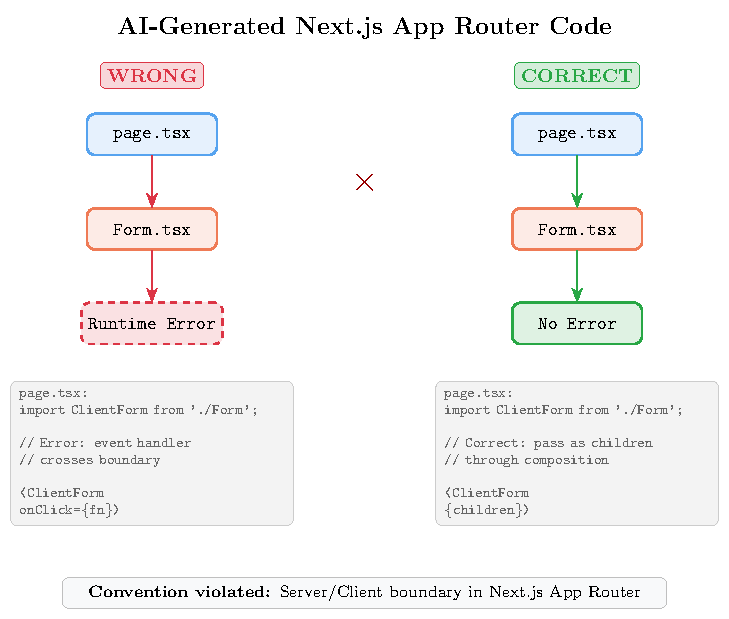
\includegraphics[width=0.88\textwidth]{figs/fig-motivated-example.pdf}
   \caption{AI-generated Next.js App Router code violating Server/Client boundaries by passing event handlers across component types, with the CORRECT panel showing the composition-pattern fix.}
   \label{fig:motivated-example}
 \end{figure}

A concrete failure mode motivates this thesis (\autoref{fig:motivated-example}). When an AI coding assistant generates a Server Component that imports a Client Component and passes an event handler as a prop, Next.js produces the runtime error ``Event handlers cannot be passed to Client Component props.'' \code{tsc --noEmit} cannot catch this, since the type system has no representation for boundary violations. During SmartKit's development I observed recurring AI generation errors in Next.js App Router code first-hand, including authentication security flaws, component boundary violations, and outdated API usage from older training data. This observation is consistent with broader surveys of AI-coding-assistant usage that document usability challenges and recurring error patterns \parencite{dakhel2023github,liang2024survey}. These are development-time observations, not measured prevalence figures.

Existing benchmarks, HumanEval and SWE-bench, score algorithmic correctness and bug-fixing capability, but none measures framework convention adherence \parencite{chen2021evaluating,jimenez2024swebench}. Hou et al.'s systematic review likewise shows, based on the metric inventory reported in that review, that framework-convention adherence is not separately tracked; generation-task metrics dominate the literature \parencite{hou2024llmse}. These metrics do not capture Next.js App Router boundaries, type-safe contracts, or file-system routing, motivating this thesis's three-dimensional framework.


\section{The Problem: AI Convention Violations in Next.js}

This thesis addresses a concrete problem: AI coding assistants can generate Next.js App Router code that violates framework conventions. The violations produce runtime errors and technical debt, yet no evaluation framework exists to measure adherence. Two design tensions shape this framework.

Framework conventions are implicit and distributed across documentation, error messages, and community patterns, so enumerating them into testable metrics is part of the design problem. AI-generated failures in Next.js also surface at runtime rather than at compile time; the example above illustrates this. This thesis measures repository-level conventions: file structure, naming patterns, and type declarations.

The focus on Next.js App Router is deliberate. Market dominance makes it the primary target: Next.js is reported at 20.8\% in the Stack Overflow 2025 Developer Survey's web-frameworks-and-technologies category, ahead of Express (19.9\%) and Angular (18.2\%) \parencite[1, Stack Overflow Developer Survey]{stackoverflow2025}. Training-data mismatch is a recognised failure mode of {LLM}-based code assistants; Wu et al.\ introduced VersiCode, a benchmark that spans hundreds of libraries and thousands of versions across multiple years, and showed that version-controllable code generation (version-specific completion and version-aware migration) remains a significant challenge even for frontier models \parencite{versicode2024}. Practical feasibility also applies: I have existing Next.js expertise, which enables direct testing of enforcement mechanisms. The pilot targets Cursor because its AGENTS.md feature implements documentation-based guidance \parencite{cursor2024docs}, an approach consistent with prior research suggesting that explicit context and structured prompts improve AI coding-assistant output quality \parencite{barke2022grounded,zhang2023practices}.

\section{Research Objectives and Questions}
\label{sec:research-objectives}

Next.js dominates React meta-framework adoption, and AI coding assistants such as GitHub Copilot and Cursor have demonstrated large productivity gains, yet no systematic evaluation framework bridges the two areas: a framework that measures how closely AI-generated Next.js boilerplate code adheres to framework-specific conventions is missing. HumanEval and SWE-bench address algorithmic problem-solving and bug-fixing capability, but none captures the architectural requirements of Next.js App Router: Server/Client component boundaries, type-safe contracts, or file-system routing conventions. This thesis targets that gap.

The primary motivation is to bridge it by designing a three-dimensional evaluation framework that turns an implicit set of framework conventions into measurable, comparable scores, and by instantiating the framework in SmartKit, a structured Next.js boilerplate that provides the necessary enforcement mechanisms and the evaluation target codebase.

The research is organised around three objectives:
{\sloppy
\begin{itemize}
    \item \textbf{Design a three-dimensional evaluation framework.}
    Construct a framework that scores AI-generated Next.js boilerplate
    code along three dimensions: Structural Integrity, Type \& Contract Safety, and
    Coverage \& Completeness, so that convention adherence becomes a quantitative,
    comparable property of generated code.
    \item \textbf{Implement SmartKit as a structured architecture.}
    The thesis releases SmartKit, an open-source Next.js boilerplate
    that demonstrates feature-based modularity, explicit Server/Client
    boundaries, and type-safe contracts, providing both the enforcement
    mechanisms and the target codebase for the framework.
    \item \textbf{Demonstrate framework applicability through a bounded
    feasibility run.} The thesis applies the framework to a representative
    feature generated by Cursor to verify that
    the framework can produce scores on real AI-generated code.
\end{itemize}
}

I address two research questions:
\begin{itemize}
    \item \textbf{RQ1:}\label{RQ1} How can an evaluation framework be consistently designed to
    measure AI coding assistant adherence to Next.js App Router boilerplate conventions along the Structural Integrity, Type \& Contract Safety, and
    Coverage \& Completeness dimensions?
    \item \textbf{RQ2:}\label{RQ2} Can the resulting framework be operationalized into measurable
    metrics, and does it demonstrate applicability when applied to
    representative AI-generated Next.js features?
\end{itemize}

These research questions are addressed through a set of framework
properties and pre-registered directional predictions, which are
defined and evaluated in Chapter~\ref{sec:evaluation}.

This thesis makes one primary contribution and two supporting
contributions. The primary contribution is a three-dimensional
evaluation framework that measures how closely AI coding
assistants follow Next.js App Router conventions. Existing
benchmarks score algorithmic correctness; this framework
measures framework-specific quality instead.

The first supporting contribution is SmartKit, an open-source
Next.js boilerplate that puts these conventions into practice;
it supplies both the conventions the framework measures and the
codebase it measures them on. The second supporting contribution
is a replicable pilot protocol comprising a pre-registration
document, a two-scaffold comparison, a scoring rulebook, and a
baseline-bootstrap script. This protocol sets up the feasibility
demonstration in Chapter~6 and the future work in Chapter~7.


\autoref{fig:evaluation-framework} summarizes the resulting evaluation-framework architecture. Each of the three dimensions is paired with an automated measurement: Structural Integrity is measured through parsed-AST rule violations, Type \& Contract Safety through TypeScript compiler output, and Coverage through a rule-coverage matrix checked against the convention catalog. The three measurements are designed to apply to a shared corpus of
AI-generated artifacts, producing a per-tool violation matrix,
type-error rates, and coverage scores. The pilot in this thesis
exercises the architecture at a smaller scale. Because the dimensions are designed as independent, no single composite score can substitute for examining all three independently. If the dimensions prove correlated in practice, reporting them separately still serves a diagnostic purpose: identifying which dimension regresses, similar to reporting precision and recall separately even when they correlate.

\begin{figure}[H]
  \centering
  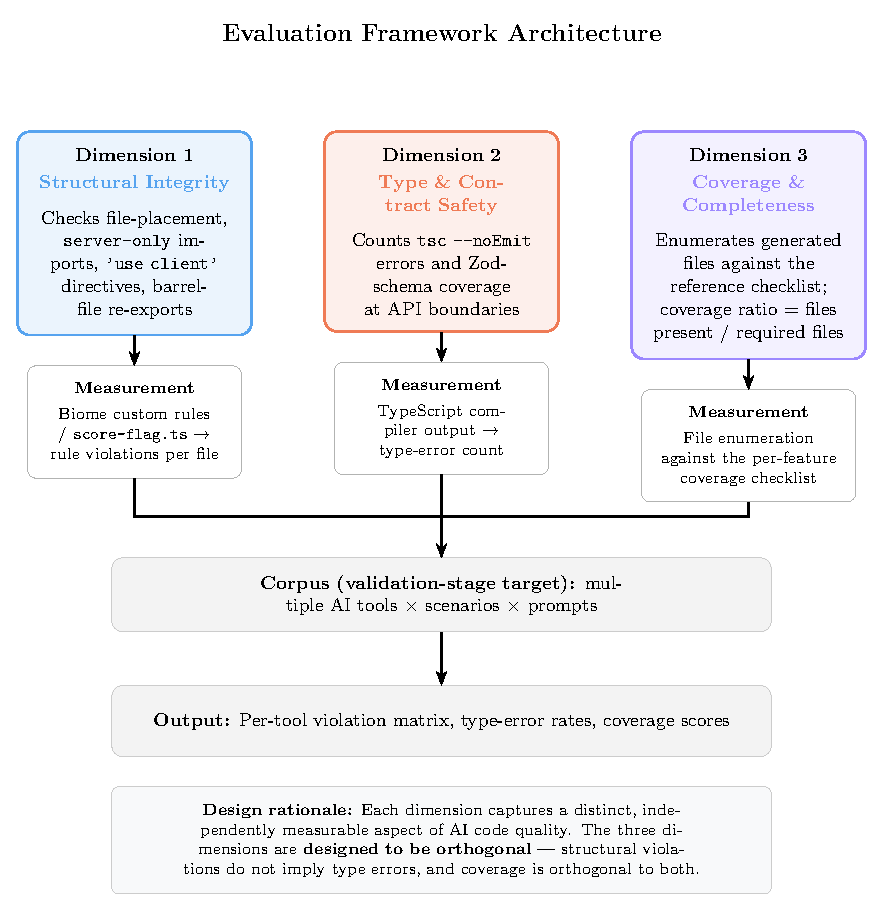
\includegraphics[width=0.88\textwidth]{figs/fig-evaluation-framework.pdf}
  \caption{Three-dimensional evaluation framework for AI-generated Next.js code: structural integrity, type safety, and coverage completeness}
  \label{fig:evaluation-framework}
\end{figure}


\section{Intended Users and Adoption Path}
\label{sec:intended-users}

SmartKit targets solo developers and small teams (two to five members) who build Next.js projects with AI coding assistants and already understand React and TypeScript. They want to reduce boilerplate setup time and keep AI-generated code consistent with project conventions. The framework supports incremental adoption: a team can adopt the feature-based folder structure and the Server/Client boundary conventions without committing to the full SmartKit stack, validating the conventions in an existing codebase before picking up billing, authentication, or email integrations.

\section{Scope and Limitations}
\label{sec:scope-limitations}

This section lists the boundaries I set before running the
pilot, the reasoning behind each boundary, and the consequence each
boundary has for the conclusions the data can support.

\begin{enumerate}
    \item \textbf{Framework scope:}
    The pilot uses Next.js App Router only and does not include
    Nuxt, Remix, SvelteKit, or any other React meta-framework. This
    boundary reflects what the SmartKit convention bundle was built
    to encode: each rule in the bundle references a Next.js-specific
    construct such as the \filename{app/} directory, the \usec{}
    directive, or route segments, so reusing the bundle on another
    framework would require translation work that I cannot justify
    inside a single-author thesis. The practical consequence is that
    framework-convention findings transfer directly to Next.js
    projects and only tentatively to adjacent frameworks that happen
    to share similar file-system routing.

    \item \textbf{AI assistants:}
    The bounded-feasibility demonstration runs on Cursor, used as an
    IDE, with MiniMax M3 as the model that generates code; Copilot,
    Claude Code, Windsurf, other coding assistants, and other models
    are not evaluated here. The consequence is that the findings
    describe how this Cursor and MiniMax M3 pairing adheres to Next.js
    conventions under the SmartKit prompt, not how coding assistants
    in general would respond to the same task.

    \item \textbf{Project type:}
    I evaluate one representative Next.js project that demonstrates
    common SaaS patterns (authentication, database access, multi-tenant
    routing, deployment configuration) rather than a sample of
    projects. A sample would have made external validity easier to
    argue for, but it would also have introduced uncontrolled
    variation across projects: differences in folder layout,
    dependency choices, and prior code all change the difficulty the
    AI sees on any given task. Holding the project constant keeps
    those variables out of the comparison. The cost is that the
    chosen project sits at a particular point in the difficulty
    range, and the pilot cannot say how the framework would behave
    on projects that look very different (a marketing site, an
    internal dashboard, a small API).

    \item \textbf{Pilot size:}
    Each condition runs five times for one task, giving ten
    predictions in total, classified by a pre-registered verdict
    rule. The sample size was the largest I could run reliably
    inside a single-author thesis timeline given the token cost of
    repeated Cursor invocations; a larger pilot was not feasible to
    fund or supervise. With ten predictions the framework can show
    whether the verdict rule separates the two conditions on a
    binary outcome, but it cannot estimate variance with any
    precision or detect small effects. Any claim that depends on
    effect size rather than direction should be treated as
    suggestive rather than confirmed; population-level statements
    about AI-assistant accuracy on Next.js conventions would need
    replication at substantially larger $N$.

    \item \textbf{Static analysis only:}
    The framework scores repository conventions through file
    structure, AST rules, and compiler output. Build execution,
    runtime behaviour, network calls, and user-visible interaction
    are all out of scope. This boundary follows from what the
    SmartKit bundle can express as deterministic rules: every rule
    in the bundle maps to something static in the repository, so the
    verifier can score it without launching a process. The
    consequence is that the framework measures whether the generated
    code would compile and follow convention, not whether it runs
    correctly under real traffic. A code generator that produces
    code which compiles and respects conventions but fails at
    runtime would still score as passing; this is a known blind spot
    and the framework does not claim to cover it.

    \item \textbf{Bundled effect:}
    The pilot measures the joint effect of the SmartKit convention
    bundle and cannot attribute results to individual conventions
    inside the bundle. A larger study that isolates each convention
    would have required holding every other variable constant
    across many more runs than this pilot could fund, and would
    also have made the comparison less reflective of how developers
    actually use the bundle (as a single unit, not convention by
    convention). Component-level ablation is left to future work.
\end{enumerate}

\section{Thesis Structure}
\label{sec:thesis-structure}

The remainder of this thesis moves from motivation to evidence across six chapters.

Chapter~2 grounds the thesis in three technical domains: AI coding assistants (Cursor, Copilot, Claude Code) and their context-aware completion mechanisms, Next.js App Router conventions (React Server Components, \usec{} directive, file-system routing), and SaaS boilerplate patterns that balance initialisation effort against code consistency.

Chapter~3 reviews code generation benchmarks (HumanEval, SWE-bench,...) and empirical productivity studies, then states the gap: no existing benchmark tracks framework-convention adherence as a distinct dimension. The chapter compares four alignment approaches (prompt engineering, fine-tuning, RAG, structural encoding) and explains why structural encoding was selected.

Chapter~4 describes SmartKit, a Next.js~16 App Router boilerplate organised by feature rather than by layer, using Drizzle for database access, Zod for contracts, and native \usec{} primitives for Server/Client boundaries. The chapter justifies each design choice and specifies the feature-directory convention that gives AI systems a narrow context window.

Chapter~5 implements SmartKit and the evaluation infrastructure. It documents the technology stack, directory layout, and feature-based organisation, then focuses on the pilot feature (\code{isEnabled(flagKey, userId?)}) that exercises structural, type-safety, and coverage conventions without coupling to external services.

Chapter~6 evaluates the result on AI-generated code. It defines a three-dimensional rubric (Structural Integrity, Type~\&~Contract Safety, Coverage~\&~Completeness), describes two conditions (SmartKit ecosystem vs.\ convention-naive scaffold), pre-registers three directional predictions, and reports results from five runs per condition. The chapter documents threats to validity and treats the bundled ecosystem effect as a known limit.

Chapter~7 collects the contributions: the evaluation framework, SmartKit substrate, pilot protocol, and honest assessment of scope. It answers RQ1 and RQ2 against pilot evidence and sets out seven future work directions.

\chapter{Background}
\label{sec:background}

Understanding the intersection of AI coding assistants and Next.js development requires grounding in three domains: AI coding tool capabilities and limitations, Next.js architectural patterns, and SaaS boilerplate design principles.

\section{AI Coding Assistants}

GitHub Copilot, Claude, and Cursor are transformer-based coding assistants that generate and revise code from project context. Cursor, used here as the IDE, draws on codebase indexing for project-wide context \parencite{cursor2024docs}; the model that generates code in this study is MiniMax M3. Copilot and Claude Code are considered as alternative tools in future work.

These assistants draw on surrounding code, comments, and project-wide signals such as Cursor's codebase indexing.

The research literature documents both strengths and limitations. Dakhel et al.\ found that {AI} assistance benefits expert developers who can filter suboptimal suggestions but may harm novice developers who lack the expertise to identify incorrect or inefficient code \parencite{dakhel2023github}. Liu et al.\ documented that ChatGPT performs better on older problems (pre-2021) than newer ones (with a reported pre-2021 advantage on the Accepted rate around the high-40-percentage-point range), yet it struggles with complex algorithms and domain-specific code, frequently generating solutions with security vulnerabilities and inefficient implementations \parencite{liu2024chatgpt}.

Zhang et al. mined Stack Overflow and GitHub Discussions and found that developers primarily use Copilot for code generation in general-purpose languages (JavaScript, Python) on VS Code, with data processing as the most common function category and difficulty of integration as the dominant limitation \parencite{zhang2023practices}. Pandey et al. documented Copilot time savings of up to 50\% in code documentation and autocompletion, and 30--40\% in repetitive coding, unit-test generation, debugging, and pair programming. The tool struggled with complex tasks, large functions, multiple files, proprietary contexts, and C/C++ code \parencite{pandey2024transforming}.

\section{Next.js Framework Architecture}

Next.js is a React meta-framework that provides server-side rendering, static site generation, and API capabilities within a unified application model. Version 13 introduced the App Router, which changed how React applications structure pages, layouts, and data fetching. Developers who learned the Pages Router encounter several App Router concepts that the older model did not surface, including Server/Client boundaries and file-system conventions for special files.

React Server Components are a core innovation in Next.js App Router. They execute exclusively on the server, which lets them access databases and sensitive operations directly without exposing logic to the client. The distinction between Server and Client components requires explicit marking through the \usec{} directive, creating a boundary that developers must manage carefully. Incorrect placement across this boundary produces runtime errors and performance degradation.

The App Router organises applications through a file-system-based routing mechanism. Each folder within the \filename{app/} directory corresponds to a route segment, with \filename{page.tsx} files defining the content for each route. Special files such as \filename{layout.tsx}, \filename{loading.tsx}, and \filename{error.tsx} provide shared UI and error handling across route hierarchies. This convention-driven structure enables rapid scaffolding but requires adherence to specific naming and placement patterns.

TypeScript integration in Next.js emphasises type safety throughout the application. The framework provides typed interfaces for page properties, API request and response objects, and data-fetching results. Achieving full type coverage requires consistent use of TypeScript patterns including generics, utility types, and strict mode configuration.

\section{SaaS Boilerplate Patterns}

SaaS applications share common requirements that boilerplate frameworks address: user authentication, database access patterns, multi-tenancy support, and deployment configurations. The economics of SaaS development favour approaches that reduce per-project initialisation effort while maintaining code quality and consistency.

Krüger and Berger documented the cost trade-offs of platform-oriented software reuse (upfront investment against amortised maintenance benefits) \parencite{kruger2020empirical}, a finding that complements Storey et al.'s framework-adoption pattern work below. The trade-off explains the appeal of well-designed boilerplate templates that amortise initialisation cost across multiple projects. Aleem et al.\ examined factors in {SaaS} architecture decisions (customization, scalability, multi-tenancy, security, integration, and fault tolerance among the dimensions they identify) \parencite{aleem2019maturity}.

Modern scaffolding approaches build on model-driven architecture principles. Inayatullah, Azam, and Anwar presented a UML-based DSML that automatically generates scaffolding CRUD code for cross-platform (web + mobile) applications from class diagrams, reducing repetitive implementation effort \parencite{inayatullah2019model}.

Drawing on Storey et al.\ and the broader framework-adoption literature, learnability, extensibility, and ease of migration are commonly cited as primary drivers of framework adoption, while framework lock-in and high configurability are commonly cited as adoption risks \parencite{storey2016frameworkadoption}.

\chapter{Related Work}
\label{sec:relatedwork}

This section surveys existing research on code generation benchmarks, empirical studies of AI-assisted development, and systematic literature reviews on AI for software engineering. The analysis identifies the specific gap this thesis addresses: the absence of framework-specific evaluation for AI coding assistants operating on Next.js boilerplate conventions.

\section{Code Generation Benchmarks}

The evaluation of AI coding assistants relies heavily on standardised benchmarks that measure code generation capability. Chen et al.\ introduced HumanEval as a foundational benchmark containing 164 hand-written programming problems with function signatures, docstrings, and unit tests \parencite{chen2021evaluating}. The benchmark evaluates models using Pass@1, Pass@10, and Pass@100 metrics. OpenAI's Codex achieved 28.8\% Pass@1 on this benchmark as of 2021, establishing a baseline for subsequent model development.

HumanEval focuses exclusively on single-function Python code generation with algorithmic and reasoning requirements. The design prioritises general programming capability over domain-specific or framework-aware generation. Yu et al.\ extended the benchmark concept with HumanEval Pro, adding self-invoking code generation tasks that require models to generate functions calling previously defined functions \parencite{yu2025humanevalpro}. Their work found that most LLMs exhibit a meaningful absolute drop on self-invoking tasks compared to standalone tasks (for example, o1-mini drops from a high-90s Pass@1 on standard HumanEval to the mid-70s on HumanEval Pro). This drop indicates that current benchmarks underestimate real-world code generation complexity.

SWE-bench marks a substantial advance in benchmark realism by evaluating AI models on real GitHub issues from popular Python repositories \parencite{jimenez2024swebench}. Each task requires understanding the issue description, locating relevant code, implementing a fix, and passing unit tests. Jimenez et al.\ found that models at the time of the paper resolved only a small fraction of issues. Claude~2 scored in the low single-digit percent range (the paper reports specific values for both BM25 and oracle retrieval setups, with oracle retrieval outperforming BM25), and GPT-4 also scored in the low single digits. The gap between benchmark performance and practical software engineering capability is reported as substantial.

Language-specific benchmarks surface further evaluation limitations. Petrukha et al.\ developed SwiftEval for Swift programming, finding that general-purpose benchmarks overestimated Swift code generation capability \parencite{petrukha2025swifteval}. Their language-specific benchmark documented substantial score drops (with the largest drops reported for the smallest open-source models, and smaller drops for frontier models) when evaluating the same models on Swift versus HumanEval-style Python problems.

To the author's knowledge (given the structured but non-exhaustive literature search described in the next section), no published benchmark systematically measures framework-convention adherence across multiple Next.js App Router conventions on a controlled corpus. The author did not conduct a separate systematic search of framework-adjacent code-generation studies (e.g., on Angular/Vue/React-adjacent benchmarks). Existing benchmarks focus on algorithmic problem-solving and bug fixes in codebases rather than framework-compliant boilerplate generation from scratch.

Several extensions and alternatives warrant mention. Liu et al.\ developed HumanEval+ and MBPP+ as rigorous extensions of the original benchmarks, finding that pass rates drop substantially on average across the LLMs they evaluated (in the roughly 20\% range) when measured against additional auto-generated high-quality tests per problem \parencite{liu2024correct}. Zhuo et al.\ introduced BigCodeBench, which evaluates a large set of fine-grained tasks (over one thousand, combining diverse function calls with complex natural-language instructions) \parencite{zhuo2024bigcodebench}. Hendrycks et al.\ proposed APPS, a 10{,}000-problem benchmark spanning introductory, interview, and competition-level coding challenges \parencite{hendrycks2021apps}. Jain et al.\ addressed the critical contamination problem through LiveCodeBench, which sources problems from recent competitive programming contests published after model training cutoffs \parencite{jain2024livecodebench}. Li et al.\ developed CodeReviewer for code review automation, an adjacent evaluation direction that assesses code quality dimensions relevant to AI-assisted development workflows \parencite{li2022codereviewer}. Each of these benchmarks measures distinct aspects of code generation or code quality capability, yet none evaluates the framework-specific convention adherence that the SmartKit framework targets.

\section{Empirical Studies on Developer Productivity}

Several empirical studies examine how AI assistance affects real developer workflows. Peng et al.\ conducted the seminal controlled experiment on GitHub Copilot with 95 recruited developers implementing an HTTP server in JavaScript \parencite{peng2023impact}. Their methodology used a treatment-control design with matched tasks, finding the 55.8\% completion time improvement cited earlier. Heterogeneous effects showed that less experienced developers benefited most from AI assistance. A large-scale survey by Liang et al.\ examined the usability of AI programming assistants and documented both successful use cases and recurring usability challenges in developer workflows \parencite{liang2024survey}.

Liu et al.\ assessed ChatGPT code generation quality across multiple languages and task types \parencite{liu2024chatgpt}. ChatGPT performs better on pre-2021 problems with a substantial pre-2021 vs.\ post-2021 advantage on Accepted rate (the paper reports a 48.14\% advantage), yet its ability to directly fix erroneous code through multi-round dialogue is relatively weak. Generated code often contained security vulnerabilities and inefficient implementations requiring human verification; the paper reports that ChatGPT resolved 89.4\% of identified vulnerabilities through multi-round fixing. In a separate comparison, the same authors found that across 728 LeetCode problems in five languages (C, C++, Java, Python3, and JavaScript), AI-generated Python3 solutions had an 8 percentage-point lower share of low-cognitive-complexity submissions than human-written solutions (42.6\% versus 50.6\% low cognitive complexity). Cyclomatic complexity distributions for Python3 closely resembled the human baseline (44.5\% versus 45.8\% low cyclomatic complexity, a 1.3 percentage-point difference), while C++ showed a 5 percentage-point offset for cyclomatic complexity (34.2\% ChatGPT versus 39.3\% human low cyclomatic complexity) \parencite{liu2024chatgpt}. Yetiştiren et al.\ separately found, in their code quality evaluation study, that ChatGPT, Copilot, and CodeWhisperer all generated code with maintainability issues, particularly improper naming and high cognitive complexity, with reported technical-debt averages of 8.9~minutes for ChatGPT, 9.1~minutes for GitHub~Copilot, and 5.6~minutes for Amazon~CodeWhisperer \parencite{yetistiren2023evaluating}.

AlOmar et al.\ analysed 17,913 developer--ChatGPT conversations about refactoring and found that developers often make generic refactoring requests (the most common pattern, observed in 41.9\% of conversations, is copy-pasting the code fragment together with a textual description of the desired fix), while ChatGPT typically includes the refactoring intention in its response \parencite{alomar2024refactoring}. The paper highlights that ChatGPT has limited understanding of the broader codebase context, leading to possible missing dependencies and code-dependencies, and that its suggestions sometimes produce compiler errors or fail tests. AI effectiveness therefore depends on the quality of the developer's prompt and on the structure of the interaction, not only on the tool itself.

Hou et al.\ conducted a systematic literature review of 395 research articles on LLMs for software engineering from 2017--2024 \parencite{hou2024llmse}. Code generation (118 papers, approximately 30\% of the corpus) and program repair (35 papers, approximately 9\%) are the two most-studied application areas. The review's metric inventory groups evaluation by problem type rather than by benchmark-versus-human split; note that the following counts refer to task instances (a single paper can address multiple task types, so the totals exceed the 395-paper corpus): 338 generation-task instances used 19 metric families (BLEU/BLEU-4/BLEU-DC in 62 studies, Pass@k in 54, Accuracy@k in 39, Exact Match in 36), 147 classification-task instances used nine metric families (Precision in 35, Recall in 34, F1-score in 33), 39 recommendation-task instances used six metric families (MRR in 15, Precision@k and F1-score@k in six each), and 1 regression-task instance used MAE. Reported effectiveness varies widely by task type. The review identified research gaps in security, requirements engineering, and empirical studies. Framework-specific boilerplate evaluation would begin to address these gaps.

Russo et al.\ developed the Human-AI Collaboration and Adaptation Framework (HACAF), which organises multiple theoretical dimensions across individual (perceived usefulness, ease of use, behavioural intention), technological (compatibility, relative advantage, complexity), and social (social influence, environmental support, self-efficacy) levels \parencite{russo2024navigating}. Technical capability is necessary but insufficient on its own; this thesis reads their analysis as indicating that human factors, including trust, skill, and workflow integration, are necessary alongside technical capability for developer-tool adoption. Evaluating framework-specific boilerplate tools therefore requires attention to how well they integrate with developer workflows and support skill development.

\section{Evaluation Methodology}

The refinement of {AI}-generated code has received attention as a complementary evaluation dimension. Liu et al.\ analyzed several thousand ChatGPT-generated programs (over four thousand programs across over two thousand programming tasks in Java and Python) \parencite{liu2024refining}. Of these programs, the majority were deemed correct, a substantial subset produced wrong outputs, a smaller subset contained compilation or runtime errors, and the remaining programs fell into additional categories; nearly two thousand programs suffered from maintainability issues identified through static analysis. Their automated refinement pipeline using static-analysis feedback improved code quality by a substantial margin (more than twenty percent). Evaluation frameworks should therefore measure both initial generation quality and the effort required for refinement.

Ouyang et al.\ studied the non-determinism of ChatGPT in code generation \parencite{ouyang2025nondeterminism}. Across 829 coding problems in three benchmarks (CodeContests, APPS, and HumanEval), the paper reports that the ratio of coding tasks with zero equal test output across different requests is substantial (47.56\% for HumanEval, 51.00\% for APPS, and 75.76\% for CodeContests, under the default temperature of 1). Setting the temperature to 0 does not guarantee determinism, despite being a common practice. Reliable assessment therefore requires multiple runs with confidence intervals rather than single-point measurements.

Beller et al.\ proposed the Diff Authoring Time (DAT) metric for measuring software development productivity at Meta \parencite{beller2025dat}. DAT measures the active work time engineers take to develop self-contained changes, using telemetry integrated with version control, IDEs, and the operating system. The team validated DAT through observational studies, surveys, visualizations, and descriptive statistics, and demonstrated its use through three case studies (a controlled experiment on mock types yielding a 14\% DAT improvement, a case study on automatic memoization in the React compiler yielding 33\% improvement, and a code-sharing estimate of $>$50\% improvement). DAT models a path for evaluating AI-boilerplate interaction that complements quantitative performance metrics with survey-based and qualitative developer experience signals.

Sauvola et al.\ projected multiple primary future scenarios for generative AI in software development, ranging from legacy integration to clean-slate and networked development, with software production shifting toward higher-level design and oversight roles as routine coding tasks become increasingly automated \parencite{sauvola2024future}. Research on optimising AI interaction patterns, including framework-specific boilerplate conventions that reduce the cognitive overhead of AI-assisted development, follows from this projection.

\section{Research Gap Summary}

The reviewed literature establishes that AI coding assistants support repetitive work, boilerplate is a suitable application area, and existing benchmarks do not measure framework-convention adherence. The structured search was non-exhaustive and did not separately survey Angular-, Vue-, or React-adjacent benchmarks. The search combined database queries on Google Scholar, arXiv, and the ACM Digital Library using terms such as ``code generation benchmark,'' ``framework convention adherence,'' and ``AI coding assistant evaluation,'' filtered by publication year (2017--2025) and citation tracking on the seed papers identified by Chen et al.~\parencite{chen2021evaluating} and Jimenez et al.~\parencite{jimenez2024swebench}. Papers that did not address a generative code task or a measurement of code quality on generated artifacts were excluded. As detailed above, Hou et al.'s review does not, according to its metric inventory, track framework-specific convention adherence as a category \parencite{hou2024llmse}. This absence in one review is not equivalent to absence in the broader literature, and the thesis therefore proposes a Next.js framework and evaluation methodology to begin addressing this gap.

\section{Alternative Approaches to AI-Codebase Alignment}

The structural approach taken by SmartKit is one of several strategies that researchers and practitioners have explored to improve AI-codebase alignment. This section reviews four alternative approaches and explains why the structural approach was selected for this thesis.

\textbf{Prompt engineering.} Few-shot prompting and chain-of-thought techniques can guide models toward framework-specific conventions by providing examples in the prompt \parencite{openai2024prompting,wei2022chain}. Prompt engineering offers flexibility and requires no model retraining. However, few-shot performance varies widely with example selection and ordering \parencite{brown2020language}, and the same prompt may produce different behaviours across different model versions, so prompts may not transfer reliably between model generations.

\textbf{Fine-tuning.} Training or fine-tuning a model on a corpus of framework-relevant code (as with general code LLMs such as Code Llama~\parencite{roziere2023code}) can embed conventions from the training distribution into model weights. Fine-tuning produces models that generate code consistent with patterns observed during training without additional prompting. However, fine-tuning requires heavy compute resources and labeled training data, and the resulting model is version-locked to the framework conventions present in the training corpus.

\textbf{Retrieval-augmented generation.} RAG retrieves relevant documentation or code examples at generation time and includes them in the model's context \parencite{lewis2020retrieval,ram2023context}. RAG provides up-to-date information without retraining and can surface framework-specific patterns from documentation. However, RAG does not enforce structure: retrieved documentation may describe conventions, but the model still decides whether to follow them.

\textbf{Structural encoding.} SmartKit encodes conventions at the project structure level through file location, naming patterns, and colocated validation schemas. Conventions are made more discoverable to AI systems through the file system rather than through external prompts or retrieved documents. This approach addresses the limitations of the alternatives: conventions are embedded in project structure rather than relying on developer vigilance, and they are reusable templates that scale across features. They evolve with the project rather than requiring model retraining. Linters operate alongside SmartKit's structural conventions rather than substituting for them: Biome 2.5.6 is included in SmartKit as a post-hoc consistency check.

The structural approach works alongside prompting and documentation, not as a replacement. The pilot evaluates whether structural conventions produce measurable behavioral change in AI assistants when combined with minimal prompting. \autoref{tbl:starter-comparison} positions SmartKit qualitatively against five established Next.js starter templates on seven dimensions relevant to AI-assisted boilerplate generation. The comparison is descriptive rather than empirical: cells summarise publicly documented features of each template, not measured outcomes, and no performance claim should be drawn from them.

\begin{table}[htbp]
\centering
\footnotesize
\renewcommand{\arraystretch}{1.3}
\setlength{\tabcolsep}{2.5pt}
\caption{Qualitative positioning of SmartKit against five established Next.js starter templates across seven dimensions.\label{tbl:starter-comparison}}
\begin{tabular}{@{}p{2.5cm}*{6}{>{\centering\arraybackslash}p{1.95cm}}@{}}
\toprule
 & \textbf{SmartKit} & \textbf{create-t3-app} & \textbf{Next.js official} & \textbf{Vercel templates} & \textbf{shadcn/ui} & \textbf{bulletproof-react} \\
\midrule
Feature-based layout & Yes & Partial & No & No & No & Yes \\
Server/Client convention & \usec{} & tRPC types & Manual & Manual & Manual & Manual \\
ORM included & Drizzle & Prisma & None & None & Drizzle & Prisma \\
Auth library & \pkg{better-}\pkg{auth} & NextAuth.js & None & NextAuth.js & Auth.js & Context API \\
TypeScript-first & Yes & Yes & Optional & Optional & Yes & Yes \\
Testing scaffold & Vitest & Vitest & None & None & Vitest & Vitest \\
AGENTS.md & Yes & No & No & No & No & No \\
\bottomrule
\end{tabular}
\renewcommand{\arraystretch}{1}
\end{table}
 

\chapter{Proposed Solution}
\label{sec:solution}

This section presents the design of SmartKit, a Next.js boilerplate built for use with AI coding assistants. The design draws on empirical findings from the literature and on domain-specific analysis of Next.js conventions, producing a codebase structure that improves AI comprehension and output quality.

This thesis uses three related but distinct terms. \textbf{SmartKit} refers to the artefact released on \href{https://github.com/Springblade/SmartKit}{\textcolor{blue}{GitHub}}: a Next.js App Router boilerplate encoding project conventions (AGENTS.md, FSD directory structure, sibling feature examples, Zod schema patterns, Biome configuration, and tsconfig path aliases). \textbf{SmartKit-style structuring condition} (abbreviated as Condition A) is the experimental condition used in the pilot, comprising AGENTS.md plus the full SmartKit feature-based layout and dependency surface. \textbf{SmartKit ecosystem} is the bundle-as-a-whole, the unit of measurement in the pilot. Findings in Chapter~6 are reported at the ecosystem level because the pilot was designed to measure the joint effect of the SmartKit bundled effect rather than to isolate any single component.

\begin{table}[H]
\centering
\caption{Terminology: SmartKit-related terms used in this thesis.}
\label{tab:smartkit-glossary}
\small
\begin{tabular}{@{}lp{4cm}p{6.5cm}@{}}
\toprule
\textbf{Term} & \textbf{Scope} & \textbf{Usage in this thesis} \\
\midrule
SmartKit & The open-source artifact & Architecture discussion (Chapters 4--5), artifact release \\
Condition A & Experimental condition using SmartKit & Pilot design \& results (\autoref{sec:pilot-protocol}) \\
SmartKit ecosystem & All priming materials (structure + AGENTS.md + examples) & Mechanism discussion, bundled-effect analysis (6.4) \\
\bottomrule
\end{tabular}
\normalsize
\end{table}

\section{Design Rationale}
\label{sec:ch4-design-rationale}

Zhang et al.\ surveyed developers and found that Copilot is primarily used for code generation in general-purpose languages (JavaScript, Python) on VS Code, with data processing as the most common function category and integration difficulty as the dominant limitation \parencite{zhang2023practices}. This finding motivates the focus on boilerplate interaction as an appropriate domain for AI enhancement. Barke et al.\ observed that programmers interact with Copilot in two modes: acceleration (Copilot executes a known plan) and exploration (Copilot helps discover APIs), with a codebook of four prompting strategies that distinguishes context-free prompts from context-aware ones \parencite{barke2022grounded}. These findings motivate three architectural decisions in the SmartKit design: encode conventions explicitly, group related code narrowly, and define type-safe contracts.

The first decision is feature-based modularity over layer-based organisation. Many Next.js projects organise code by technical layer (\filename{components/}, \filename{lib/}, \filename{hooks/}) or by page. Layer-based organisation creates wide import graphs: a single component may transitively import from dozens of files, so an AI system generating a new component receives a large, undifferentiated context. Feature-based modularity confines all code for one feature (schemas, actions, components, emails, types) within a single directory, giving the AI a narrow, self-contained context window. The trade-off is that cross-cutting concerns (shared utilities, types, or components) require deliberate extraction to a shared layer. I judge this overhead acceptable for SaaS boilerplate where the feature boundary is the primary decomposition axis.

The second decision is Drizzle ORM over Prisma. Prisma uses a schema-first DSL (\filename{.prisma} file) that generates a client. Drizzle uses a TypeScript-first schema directly in \filename{.ts} files, colocated with the application code. I considered Prisma first because the schema-first DSL is easier to onboard onto. Then I read three RealWorld-tier codebases that mixed Prisma schemas with TypeScript business code, and the boundary confused the AI in every case. Drizzle's TypeScript-first approach won out for this thesis despite the steeper SQL learning curve: with Drizzle the AI reads and extends the schema using the same language model it uses for the rest of the codebase. Schema changes propagate through TypeScript's own type inference without a separate code-generation step.

The third decision is explicit Server/Client boundaries over tRPC-based type sharing. tRPC provides end-to-end type inference across the Server/Client boundary by sharing a single TypeScript interface definition. This eliminates a class of type errors but requires a separate router definition and does not enforce the architectural boundary at the file level. SmartKit instead uses Next.js's native \usec{} directive for Client Components and the \pkg{server-only} import \parencite{server-only-npm} for server-only utilities, supplemented by Zod schemas shared across the boundary. The native mechanism is framework-default rather than library-specific, so the conventions survive beyond the SmartKit codebase and transfer to plain Next.js projects; tRPC conventions do not transfer the same way. The trade-off is that the native mechanism requires explicit developer discipline; tRPC enforces the boundary automatically through its type system. Per-feature Zod schemas are colocated under \filename{features/<name>/types/} so the same definition is the source of truth for both runtime validation (server action) and TypeScript inference (client component props).

\section{Feature-Based Modular Architecture}

Many Next.js projects organize code by technical layer (components/, lib/, hooks/) or by page structure. SmartKit instead uses feature-based modularity, where each feature contains everything needed for its functionality: an authentication feature, for instance, holds database schemas, API routes, React components, form validation schemas, and email templates inside one directory.

This organization makes AI context retrieval more focused by narrowing the search space to relevant feature-specific files when code is generated for one feature. The scope of any change becomes explicit, which may reduce the risk of AI-generated code violating feature encapsulation. The directory boundary is also a natural test and deployment unit that matches developer mental models.

The feature directory structure follows a consistent pattern across all features:

\begin{lstlisting}[
  language={},
  caption={Feature directory layout convention used across SmartKit.},
  label={lst:feature-layout},
  basicstyle=\ttfamily\small,
  showstringspaces=false,
]
src/features/{feature-name}/
+-- components/         # React components
+-- lib/               # Feature-specific utilities
+-- types/             # TypeScript type definitions
+-- emails/            # Email templates
+-- index.ts          # Public API barrel
\end{lstlisting}

This structure allows AI systems to predict where to place new code within a feature, reducing the cognitive overhead of project organization.

\section{Server/Client Boundary Conventions}

React Server Components introduce an explicit boundary between server-only and client-accessible code. SmartKit relies on Next.js's native mechanism (the \usec{} directive and the \pkg{server-only} import) rather than a library such as tRPC, because the native mechanism is framework-default and makes Server/Client boundary violations surface as build-time failures that the rubric can read. This section focuses on how those two primitives are applied in practice: where they live in the source tree, and what data-flow shape they impose on AI-generated code.

The boundary shapes data-flow design. Server Components can read databases and environment variables directly, while Client Components receive data through props or invoke server actions. AI systems can therefore call type-safe server actions from a Client Component, which keeps the data path consistent as new components are generated.

\autoref{lst:agents-md} shows a representative excerpt from the SmartKit \filename{AGENTS.md} file, which encodes the conventions that Cursor reads when operating inside the project. The file defines project-level rules that are intended to be persistent and high-priority within Cursor's instruction hierarchy, and includes specific conventions for file placement, Server/Client boundaries, and schema sharing. The pilot does not independently confirm the relative priority of AGENTS.md rules versus inline comments or tool outputs.

\begin{lstlisting}[
  language={},
  caption={Representative excerpt from SmartKit's AGENTS.md file.},
  label={lst:agents-md},
  basicstyle=\ttfamily\small,
  showstringspaces=false,
]
# SmartKit Boilerplate: Code Conventions

Rules for AI coding assistants working inside smartkit/.

## Project Shape
- Next.js 16 App Router, TypeScript 5.7.3 strict mode
- Feature-based layout: all feature code lives under src/features/{name}/
- Zod 4 for schema validation, Drizzle ORM for the database, Biome for lint/format
- Vitest + Testing Library + Happy DOM for tests
- Authentication via Better Auth; email via Resend + React Email templates

## Feature Directories
- Place all feature code under src/features/{name}/
- Default subdirectories: components/, hooks/, actions/, lib/, types/, emails/
- Strong default, not enforcement: single-file features may live at the feature root

## Server/Client Boundaries
- Client Components: 'use client' directive at the top of the file
- Server-only utilities: server-only import to prevent client bundling
- Do not use .server.ts / .client.tsx filename conventions

## Schema Sharing
- Zod schemas are defined once in the feature types/ directory
- The same schemas validate payloads on the client before submission and on
  the server inside route handlers and server actions
- Keep type definitions explicit; avoid any types
\end{lstlisting}

\section{Database Schema Patterns}

SmartKit uses Drizzle ORM with PostgreSQL to provide type-safe database access across the application. The schema design follows conventions that AI systems can learn from existing tables and reproduce for new ones: each table declares columns with explicit types, relations through foreign keys, and indexes for query optimisation.

The Drizzle query pattern lets AI-generated code read and write the database through type-safe query builders. AI systems can examine an existing schema to infer a join or insert shape and produce code that preserves type safety end-to-end. Ad-hoc queries that bypass type checking or violate the file-level conventions are discouraged.

Better~Auth supplies the shared identity tables (user, session, account, verification) used by every feature that signs users in, while \filename{features/billing/} owns its own \code{billing} and \code{payment\_transactions} tables. All four Better~Auth tables and the billing tables live in \filename{src/database/schema/}, one infrastructure directory outside the FSD hierarchy, with relations declared in \filename{src/database/schema/relations.ts}. The single-directory placement lets \pkg{drizzle-kit} scan every schema in one pass and lets any feature import shared row types (\filename{database/schema/index.ts}) without depending on a sibling feature. The placement keeps database patterns centralised while still being directly importable from any feature module.

\section{Type-Safe API Contracts}

API routes in SmartKit use Zod schemas for request and response validation, parsed at the route handler and reused on the client via \pkg{z.infer}. The AI can read and extend the same Zod syntax it encounters in existing features such as \filename{features/billing/} and \filename{features/auth/}. The pilot feature itself has no API route; the Contract Safety sub-score instead checks whether \code{FlagKey} is derived from a Zod schema at the function boundary, as noted in \autoref{sec:integrations-and-pilot}.

\chapter{Implementation}
\label{sec:implementation}

This chapter documents how SmartKit's design choices turn into a working Next.js~16 project. The first section covers the stack and directory layout; the second walks through the feature flag utility and the scoring script; the third briefly notes the billing integration that the pilot does not exercise.

SmartKit already ships with a feature directory layout and Zod schemas. These give the pilot its Condition~A patterns. The artifact also includes billing, authentication, and email integrations, which makes it usable as a SaaS boilerplate. The pilot feature itself calls none of these services. Section~\ref{sec:integrations-and-pilot} details the distinction between patterns the AI can see and services the generated feature actually exercises.

\section{Technology Stack}
\label{sec:technology-stack}

This section documents the SmartKit stack and the directory layout the rubric reads. The dependency choices below support the artifact and the comparison described in chapter 6.

\subsection{Stack selection rationale}
\label{sec:stack-rationale}

Each component of the SmartKit stack reinforces one of the three evaluation dimensions.

Next.js~16's App Router exposes the conventions Structural Integrity measures: Server and Client boundaries, file-system routing, and the \usec{} directive paired with the server-only import. These rules transfer to plain Next.js projects rather than coupling the rubric to library-specific ones. Zod~4 and TypeScript~5.7.3 strict mode jointly serve Type~\&~Contract Safety; \code{tsc --noEmit} gives the compile-time signal. Zod schemas, colocated under \filename{features/<name>/types/}, are parsed at the Server Action boundary and reused on the client via \pkg{z.infer}. One schema then becomes the source of truth on both sides, and Coverage~\&~Completeness can check for its presence at the expected path. Server/Client boundary errors surface as build-time failures that Structural Integrity reads. A tRPC-style shared router would hide the boundary inside library types and remove that signal. SmartKit uses framework-native primitives to keep that signal visible.

\subsection{Dependency version pins}
\label{sec:dependency-pins}

Table~\ref{tbl:dependency-pins} lists the canonical versions of the libraries in the stack. Versions are pinned to the values declared in \filename{smartkit/package.json} at the snapshot used for the pilot evaluation.

\begin{table}[H]
  \centering
  \small
  \caption{Canonical dependency pins for SmartKit at the pilot-evaluation snapshot.}
  \label{tbl:dependency-pins}
  \begin{tabular}{ll}
    \hline
    \textbf{Dependency} & \textbf{Version} \\
    \hline
    Next.js & 16.2.12 \\
    React / React DOM & 18.3.1 \\
    TypeScript & 5.7.3 \\
    Drizzle ORM & 0.45.2 \\
    Zod & 4.4.3 \\
    Biome & 2.5.6 \\
    Tailwind CSS & 4.3.3 \\
    Resend & 6.18.1 \\
    React Email & 6.9.1 \\
    better-auth & 1.6.x \\
    Vitest & 4.1.x \\
    \hline
  \end{tabular}
\end{table}

Next.js~16.2.12 supplies the App Router architecture. Drizzle~ORM~0.45.2 (PostgreSQL) and Zod~4.4.3 jointly enforce the type-safe-contract principle described above. The remaining tools are consistency choices. Tailwind~CSS~4.3.3 (CSS-first configuration) handles styling, Biome~2.5.6 acts as a single linter and formatter, Resend~6.18.1 with React~Email~6.9.1 powers transactional email templates, and SePay integrates as the payment gateway through \filename{features/billing/} (HMAC signature verification plus idempotent webhook handling; the implementation is described in the billing subsection). \pkg{@better-auth/drizzle-adapter} ties authentication to the database layer.

\subsection{Project structure}
\label{sec:project-structure}

The SmartKit project structure implements the feature-based architecture.

\subsubsection{Top-level directory layout}
\label{sec:top-level-layout}

\begin{figure}[htbp]
  \centering
  \begin{forest}
    dirtree
    [\textbf{smartkit/}
      [src/
        [app/\dtnote{Next.js App Router pages}]
        [features/
          [auth/\dtnote{authentication feature}
            [components/\dtnote{React components}]
            [emails/\dtnote{email templates}]
            [lib/\dtnote{auth-specific helpers}]
            [types/\dtnote{auth type definitions}]
            [index.ts\dtnote{public API barrel}]
          ]
        ]
        [database/\dtnote{Drizzle schema, migrations, client}
          [schema/\dtnote{Better Auth + billing tables}]
          [migrations/\dtnote{Drizzle migration files}]
          [db.ts\dtnote{Drizzle client}]
        ]
        [lib/\dtnote{shared utilities}]
        [config/\dtnote{site and environment config}]
      ]
    ]
  \end{forest}
  \caption{Top-level directory structure of the SmartKit instantiation.}
  \label{fig:project-structure}
\end{figure}

Pages and layouts live in \filename{src/app/} because Next.js~16's App Router reads that path as the routing surface. Routes import feature modules from \filename{src/features/}, and feature modules never import the other way around. The page-versus-feature separation is then enforceable by static analysis: the Structural Integrity rubric can inspect server-only imports, \usec directives, and file-system routing directly from the framework's own conventions. A feature module that imports from a route would invert the dependency direction the App Router expects, and the build would fail.

The four Better Auth tables (\filename{user.ts}, \filename{session.ts}, \filename{account.ts}, \filename{verification.ts}), the relations graph in \filename{relations.ts}, and the billing tables (\filename{billing.ts} with \code{payment\_transactions}) all live in \filename{src/database/schema/} because \pkg{drizzle-kit} scans a single configured root for migrations. Any feature can import shared row types from \filename{database/schema/index.ts} without depending on a sibling feature's directory. The \filename{database/db.ts} client lives in the same place for the same reason. The \pkg{pg} pool, the \filename{env.DATABASE\_URL} read, and the schema registration all sit in one file. This keeps the runtime surface that Type~\&~Contract Safety checks via \code{tsc --noEmit} minimal and central.

Generic cross-feature helpers, including the \code{cn} class-name helper and the typed \filename{env.ts} reader, go in \filename{src/lib/} so shared utilities do not create dependencies between feature directories.

The \filename{features/flags/} directory sits at the repository top level rather than inside \filename{src/}. AGENTS.md's rule for feature-named directories does not require a \filename{src/} prefix, and keeping \filename{features/flags/} at the top lets the AI encounter it immediately when it scans the repo root.

Internally, \filename{features/flags/} follows the same conventions as \filename{src/features/auth/}. \filename{lib/} holds the \code{isEnabled} implementation, \filename{types/} holds the Zod-derived \code{FlagKey} schema, and \filename{index.ts} is the public API barrel. The unit test lives at \filename{src/tests/features/flags/is-enabled.test.ts}, following the centralized-test convention in AGENTS.md.

\subsection{Feature-based organization}
\label{sec:feature-organization}

Each feature reuses the six-subdirectory convention introduced above (\filename{components/}, \filename{hooks/}, \filename{actions/}, \filename{lib/}, \filename{types/}, \filename{emails/}). Structural Integrity reads this layout as a per-feature boundary marker.

\begin{figure}[htbp]
  \centering
  \noindent
  \begin{minipage}[t]{0.40\textwidth}
    \vspace{0pt}
    \begin{forest}
      dirtree
      [\textbf{flags/}
        [lib/
          [is-enabled.ts\dtnote{server-only}]
        ]
        [types/
          [flags.ts\dtnote{Zod schema}]
        ]
        [index.ts\dtnote{barrel export}]
      ]
    \end{forest}
  \end{minipage}%
  \hfill
  \begin{minipage}[t]{0.60\textwidth}
    \vspace{0pt}
    \begin{forest}
      dirtree
      [\textbf{src/features/auth/}
        [components/\dtnote{'use client'}]
        [hooks/]
        [actions/\dtnote{server actions}]
        [lib/\dtnote{server-only}]
        [types/\dtnote{Zod schemas}]
        [emails/]
        [index.ts\dtnote{barrel export}]
      ]
    \end{forest}
  \end{minipage}
  \caption{SmartKit's feature-based folder layout.}
  \label{fig:fsd-structure}
\end{figure}

\section{Core Feature Implementation}
\label{sec:core-feature-implementation}

This section details three core patterns the evaluation rubric targets.

\subsection{Feature flag resolution}
\label{sec:feature-flag-resolution}

The feature flag system resolves override sources in priority order: per-user overrides, then environment variables, then a static default. The implementation lives in \filename{features/flags/lib/is-enabled.ts}, which carries the \pkg{server-only} marker so Next.js fails the build if a Client Component imports it.

The Zod schema below defines the allowed \code{FlagKey} values. The schema lives in \filename{features/flags/types/flags.ts} and is reused on both sides of the boundary through \pkg{z.infer}. When the function is called, the runtime parses the input against this schema before any cache lookup.

\begin{lstlisting}[
  language=TypeScript,
  caption={Zod schema and three-tier resolution skeleton for \code{isEnabled}.},
  label={lst:is-enabled-impl},
  basicstyle=\ttfamily\scriptsize,
]
import "server-only";
import { z } from "zod";
import { FlagKeySchema, type FlagKey } from "../types/flags";

const TTL_MS = 5 * 60 * 1000;
const cache = new Map<string, { value: boolean; expires: number }>();

export function isEnabled(
  flag: unknown,
  fallback = false,
  userId?: string,
): boolean {
  const key = FlagKeySchema.parse(flag); // throws on invalid key
  const cacheKey = `${key}__${userId ?? ""}`;
  // ... read per-user override, then env, then fallback;
  // ... cache the resolved value for TTL_MS.
}
\end{lstlisting}

\textit{Design rationale.} The tiered design supports gradual rollouts through environment variables before per-user targeting. The 5-minute TTL bounds memory growth while keeping flag values fresh for environment-driven rollouts. The schema is the single source of truth for \code{FlagKey}: the same object is exported as a TypeScript type via \pkg{z.infer}, so the runtime check and the compile-time type come from one declaration.

\subsection{Server/Client boundary enforcement}
\label{sec:server-client-boundary}

The boundary rationale, including why SmartKit uses \pkg{server-only} and \usec{} instead of a library such as tRPC. The practical rule is short: a module marked import "server-only" cannot be imported into Client Components. Next.js enforces this at build time. The build-time error is the signal the Structural Integrity dimension reads.

\subsection{Evaluation infrastructure}
\label{sec:eval-infrastructure}

The framework includes an automated scoring script (\filename{scripts/score-flag.ts}) that reads source files and computes a 0--5 score per dimension. The script is read-only: it does not mutate the run directory, and it does not call any AI or LLM for scoring.

The Structural Integrity scoring function takes the run directory as input, scans TypeScript files for the \code{isEnabled} export, and classifies the file path. The pseudocode below summarizes the path-detection logic; the full implementation lives in the repository.

\begin{lstlisting}[
  language=TypeScript,
  caption={Path-detection pseudocode for Structural Integrity scoring.},
  label={lst:scoring-logic},
  basicstyle=\ttfamily\scriptsize,
]
// scoreStructural(runDir):
//   locate the file exporting isEnabled
//   if path is under features/flags/lib/         -> path_match = 1
//   if path is under features/ but wrong subdir  -> path_match = 0.5
//   if path is under app/ or root lib/           -> path_match = 0
//   feature_complete = (server-only present && barrel re-exports)
//   score = round((pathMatch + featureComplete) * 2.5)
\end{lstlisting}

The full rubric implementation lives in \filename{smartkit/scripts/score-flag.ts}. Table~\ref{tbl:scoring-summary} maps each scoring function to the dimension it reads.

\begin{table}[H]
  \centering
  \small
  \caption{Scoring functions and the dimension each one reads.}
  \label{tbl:scoring-summary}
  \begin{tabular}{lll}
    \hline
    \textbf{Dimension} & \textbf{Input signal} & \textbf{Output} \\
    \hline
    Structural Integrity & \code{tsc}-free path detection & 0--5 \\
    Type \& Contract Safety & \code{tsc --noEmit} errors + \code{: any} count & 0--5 \\
    Coverage \& Completeness & file-enumeration against checklist & 0--5 \\
    \hline
  \end{tabular}
\end{table}

\section{Billing and SePay integration}
\label{sec:billing-sepay}

The \filename{features/billing/} feature implements a payment and order-management flow backed by SePay, a Vietnamese payment gateway. The pilot feature does not exercise SePay; this section records the integration for completeness.

SePay webhook handling relies on two mechanisms. First, \filename{signature.ts} verifies the HMAC-SHA256 signature on incoming webhooks and rejects requests whose timestamp drifts more than five minutes from the server clock. Second, \filename{payment-transactions.ts} deduplicates deliveries through a unique index on the transaction id, so repeated delivery attempts under transient failures produce a no-op rather than duplicate side effects. The combination means the billing path is safe under retries without requiring the upstream gateway to track delivery state.

In Condition~A, the AI sees \filename{features/billing/} alongside \filename{features/auth/} and uses both as convention anchors when generating the pilot feature, supplementing the explicit AGENTS.md rules. Section~\ref{sec:integrations-and-pilot} discusses the billing feature's relation to the pilot evaluation. The integration has not been independently audited for security, load, or test coverage.

Taken together, the implementation choices in this chapter give the pilot evaluation a fixed substrate to measure against: a stack with pinned versions, a feature-based directory layout, a server-only boundary, a Zod-derived contract, and a deterministic scoring script. Chapter~6 reports the scores that this substrate produces across the two conditions.

\chapter{Evaluation}
\label{sec:evaluation}

This section proposes the evaluation framework and pilot feasibility study for assessing AI coding assistant performance on Next.js boilerplate generation tasks. The framework design is accompanied by a pilot evaluation protocol that exercises the framework on a representative feature.

\section{Evaluation Framework}
\label{sec:evaluation-framework}

\paragraph{Pilot claims.}
\label{sec:pilot-claims}
The pilot addresses the research questions stated in \autoref{RQ1} and \autoref{RQ2} through two classes of
claims, both pre-registered before any run was executed. \autoref{RQ1} asks whether the framework can be designed consistently along three dimensions; the framework properties (FP) below operationalise the answer. \autoref{RQ2} asks whether the framework can be applied to real AI-generated code; the directional predictions (DP) provide the falsifiable test.

\begin{description}
  \item[Framework properties (FP)] describe what the framework can
    measure. Each property claims that a dimension can produce a
    per-run score on a real artefact. The pilot supports or fails to
    support these claims; it cannot refute them.
  \item[Directional predictions (DP)] are falsifiable hypotheses
    comparing Condition~A with Condition~B. Each prediction states which
    condition is expected to score higher on a given dimension. The
    pilot classifies each prediction with the verdict rule in
    \autoref{sec:pilot-verdict}.
\end{description}

\begin{table}[H]
\centering
\footnotesize
\renewcommand{\arraystretch}{1.3}
\caption{Mapping between framework properties (FP) and directional predictions (DP).}
\label{tab:fp-dp-mapping}
\begin{tabular}{@{}p{1.2cm}p{4.5cm}p{1.2cm}p{5.5cm}@{}}
\toprule
\textbf{Property} & \textbf{Framework Property} & \textbf{Prediction} & \textbf{Directional Prediction} \\
\midrule
FP1 & Modular file layout enforced by \filename{features/} convention & DP1 & SmartKit condition produces correct \filename{features/<name>/} placement (Structural Integrity dimension); Condition~B does not \\
\midrule
FP2 & Zod schemas colocated with features as reusable contracts & DP2 & SmartKit condition produces Zod-derived types (Type \& Contract Safety dimension); Condition~B produces raw type aliases \\
\midrule
FP3 & Centralized test directory structure \filename{src/tests/features/} & DP3 & SmartKit condition places test files at predicted path (Coverage \& Completeness dimension); Condition~B places tests elsewhere or omits them \\
\bottomrule
\end{tabular}
\end{table}

\subsection{Three Dimensions}
\label{sec:dimensions}

The evaluation uses a multi-dimensional quality framework that captures different aspects of boilerplate quality. This framework extends existing benchmark methodology to address framework-specific concerns that existing evaluations overlook; the specific literature gap that motivates this framework is documented in chapter 3. SmartKit's contribution is to instantiate the missing framework-specific convention-adherence measurement dimension for Next.js App Router.

A single composite score would mask which dimension is regressing, so the framework reports each dimension separately. I assert orthogonality at design stage; Pearson correlation analysis on $n \geq 30$ per condition would distinguish genuine orthogonality from subtle coupling, and that analysis is part of the validation-stage work described at the end of this thesis.

The three dimensions capture distinct, non-overlapping aspects of boilerplate quality that affect real-world usability. Rather than measuring only output correctness, the framework assesses whether generated code can be integrated into production codebases without convention violations or type safety issues. Each dimension maps to an automated measurement approach and corresponds to a specific failure mode observed in AI-generated Next.js code.

\paragraph{Unit of analysis.}
Scoring is run-level: each run receives one aggregate score per dimension. For Structural Integrity, the score captures path correctness of the primary utility file, including required exports, \pkg{server-only} boundaries, and barrel re-exports. For Type \& Contract Safety, the score combines type-error counts with schema-validation presence under weakest-link aggregation. For Coverage \& Completeness, the score enumerates file presence against the reference checklist. The aggregation reflects that structural and contract properties are feature-level rather than file-level.

\textbf{Structural Integrity} assesses whether generated code follows Next.js conventions for file location, naming, Server/Client component boundaries, and App Router patterns. Automated checking uses the \filename{score-flag.ts} script. The dimension captures violations such as incorrect file placement in the \filename{features/} directory, missing \usec directives on client components, and non-standard naming patterns that break routing.

\textbf{Type \& Contract Safety} combines two sub-scores on the 0--5 rubric. The Type Safety sub-score reads \code{tsc --noEmit} error counts and \pkg{@typescript-eslint/}\pkg{no-explicit-any} occurrences; these indicate whether generated code introduces type regressions. The Contract Safety sub-score measures whether generated code defines typed validation schemas (Zod) for its primary contracts. For features with API routes, this captures request/response contract validation; for the pilot feature (a client-side utility), this captures whether the \code{FlagKey} type is derived from a Zod schema versus a raw TypeScript type alias. The measurement principle (typed schemas versus raw types) applies regardless of boundary type. The two sub-scores combine under the lower-of rule: the dimension score equals the smaller of the two sub-scores.

\textbf{Coverage \& Completeness} evaluates whether generated boilerplate includes all necessary artifacts for a functional feature. \autoref{tbl:coverage-checklist} shows the reference checklist for the \code{isEnabled} feature flag utility used in the pilot. Completeness is measured by enumerating generated files against the checklist and computing a coverage ratio. The pilot-feature ceiling (levels 0--3) and its rationale are documented in the pilot methodology section; levels 4--5 require integration-dependent artifacts that this feature structurally excludes by design.

\begin{table}[ht]
\centering
\footnotesize
\renewcommand{\arraystretch}{1.25}
\caption{Reference coverage checklist for the \code{isEnabled} feature flag utility.}
\label{tbl:coverage-checklist}
\begin{tabular}{@{}p{0.7cm}p{3.3cm}>{\raggedright\arraybackslash}p{9cm}@{}}
\toprule
\# & Artifact & Expected path \\
\midrule
1 & Core utility function & \filename{features/flags/lib/is-enabled.ts} \\
2 & Zod schema and FlagKey enum & \filename{features/flags/types/flags.ts} \\
3 & Unit test file & \filename{src/tests/features/flags/is-enabled.test.ts} \\
4 & Public API barrel & \filename{features/flags/index.ts} \\
5 & Cache implementation & Embedded in \filename{is-enabled.ts} (5-minute in-memory cache) \\
\bottomrule
\end{tabular}

\renewcommand{\arraystretch}{1}
\end{table}

\newpage 

\subsection{Rubric Interpretation}
\label{sec:rubric-interpretation}

The three rubric dimensions introduced and detailed in this chapter carry different epistemic statuses with respect to the underlying constructs they are taken to represent. This subsection makes those statuses explicit so that pilot results are read within the framework's validated scope, and not beyond it.

\paragraph{Three epistemic statuses.}
The three rubric dimensions carry different epistemic statuses with respect
to the underlying constructs they represent. \emph{Structural Integrity} is
\emph{measured}: scores reproduce directly from file artefacts and
compile-time signals. \emph{Type \& Contract Safety} is a \emph{proxy}: it
tracks type-error counts and Zod schema presence as a justified indicator,
but the level cutoffs have not been calibrated against downstream developer
experience. \emph{Coverage \& Completeness} is \emph{aspirational}: the
rubric predicts developer experience without empirical validation. Pilot
results should be read within the framework's validated scope, and not
beyond it. This epistemic distinction motivates the pre-registered,
directional verdict rule in \autoref{sec:pilot-verdict} rather than a
two-sided test of ``works'' versus ``fails'': a proxy score cannot refute
a hypothesis, and an aspirational score cannot confirm one either. 

\subsection{Evaluation Design: Rationale and Trade-offs}
\label{sec:design-rationale}

The design prioritises a reproducible, feasible comparison. It uses a six-level (0--5) rubric per dimension, with cutoffs defined in the rubric tables. The cutoffs are design choices and have not been calibrated against developer-experience data. The study only focuses on Next.js to maintain depth over breadth. The pilot uses automated scoring; manual or LLM-as-judge assessment remains future work. Productivity metrics such as diff authoring time and developer-reported productivity \parencite{beller2025dat} are not collected in the current pilot. The executed pilot reports only per-run time-to-correct (ttc, in minutes) as a coarse timing signal (a single wall-clock reading per run rather than a calibrated productivity measure), separate from the rubric dimensions.

Quantitative metrics derive from automated analysis of generated code. \textit{Structural Integrity} uses file-enumeration and regex detection of \usec/\pkg{server-only} usage and \filename{features/} path placement; \textit{Type \& Contract Safety} uses \code{tsc --noEmit} output and Zod schema detection; \textit{Coverage \& Completeness} uses file enumeration against a reference checklist per feature type. The complete scorer is \filename{scripts/score-flag.ts}.

\section{Pilot Methodology}
\label{sec:pilot}
\label{sec:pilot-protocol}

This section describes the pilot design. It covers the two conditions being compared, the standardised task, the scoring rubric, and the decision rule for interpreting results.


\subsection{Pilot Feature and Measurement Scope}
\label{sec:integrations-and-pilot}

SmartKit contains billing (SePay), authentication (Better~Auth), and email (Resend) integrations as part of its role as a usable SaaS boilerplate. The pilot deliberately uses a feature-flag utility that calls none of these services. The boundary isolates convention adherence from sibling-code learning and service-integration confounding, and it is the basis for the Coverage ceiling noted above. The feature was chosen for convention-representativeness, not SaaS-completeness. It requires deliberate file placement (Dimension~1: Structural Integrity), Zod contract definition and export (Dimension~2: Type \& Contract Safety), and test file creation in the correct directory (Dimension~3: Coverage \& Completeness). Billing, authentication, and email integration were intentionally excluded to avoid confounding \emph{sibling-code learning} (copying patterns from existing integrations) with \emph{convention adherence from structural encoding}. The artifact contributions stand independently of the pilot evaluation, so the comparison isolates the convention envelope without depending on whether the integrations themselves pass muster.

Condition~A exposes the full file tree, so the AI can pattern-match feature folders, colocated actions and schemas, and \pkg{server-only} boundaries. Condition~B exposes none of these convention sources. The comparison measures the bundled convention envelope, while the integrations remain evidence of SmartKit's separate artifact contribution. This bundled effect is discussed in \autoref{sec:dp2-results}.

The prompt's per-user database override is intentionally stubbed: \seqsplit{readUserOverride} returns \code{undefined} without querying Drizzle or external persistence. This keeps the resolution order testable while imposing the Coverage ceiling at levels 0--3; the design-stage limitation and score correction are documented in \autoref{sec:measurement-validity}.

\paragraph{Measurement scope.}
The Contract Safety sub-score measures API request and response contract validation in general. The pilot feature (\code{isEnabled(flagKey, userId?)}) is a client-side utility without API routes. For the pilot, Contract Safety measures schema validation at function boundaries: whether \code{FlagKey} is derived from a Zod schema rather than a raw type alias. The choice isolates convention adherence from service-integration confounding. Full API contract validation measurement is deferred to validation-phase studies with server-action or route-handler features.

The representative feature exercises none of SmartKit's integrated services. All evaluations use multiple runs to address non-determinism concerns raised by Ouyang et al.\ \parencite{ouyang2025nondeterminism}; the Cursor tool does not expose user-settable temperature, so multi-run evaluation substitutes for temperature variation.

\subsection{Conditions}
\label{sec:pilot-conditions}

\autoref{tbl:condition-ab} summarises the two conditions. Condition~A is SmartKit at full setup; Condition~B is a convention-naive Next.js scaffold produced by \code{create-next-app} with the same dependency surface but no FSD layout, no AGENTS.md, and no \filename{.cursor/rules/} folder. Both conditions keep the same dependencies (Drizzle, Resend, Better~Auth, Zod, Biome); they differ only in convention encoding (AGENTS.md, FSD layout, Zod colocation, server-only boundaries). Holding the dependency surface constant makes the comparison a matched-control one. 

\begin{table}[H]
\centering
\small
\renewcommand{\arraystretch}{1.2}
\caption{Condition~A (SmartKit at full setup) vs.\ Condition~B (convention-naive scaffold) used in the pilot evaluation.}
\label{tbl:condition-ab}
\begin{tabular}{@{}p{2.6cm}p{5.6cm}p{5.6cm}@{}}
\toprule
\textbf{Dimension} & \textbf{Condition~A (treatment)} & \textbf{Condition~B (control)} \\
\midrule
Stack surface
  & SmartKit (Next.js 16, Drizzle, Biome, Zod, Resend, Better~Auth)
  & create-next-app scaffold + full SmartKit dependency surface (Next.js 16, TypeScript, Tailwind CSS, Biome, Drizzle ORM, Zod 4.4.3, Resend, Better Auth); no \filename{src/features/} layout, no AGENTS.md, no \filename{.cursor/rules/} \\[4pt]
\midrule
Convention envelope
  & FSD \filename{src/features/<name>/}, AGENTS.md, \pkg{server-only}, colocated Zod in \filename{types/}, Server Actions in \filename{actions/}
  & No AGENTS.md, no \filename{src/features/}, flat \filename{lib/} at root \\[4pt]
\midrule
Folder layout
  & Feature-scoped: \filename{components/}, \filename{hooks/}, \filename{actions/}, \filename{lib/}, \filename{types/}, \filename{emails/} per feature
  & \filename{app/} (pages), \filename{lib/} (flat), \filename{components/} (flat) \\[4pt]
\midrule
AI tool context
  & Sees existing \filename{features/auth/}, \filename{features/billing/} patterns; conventions live in repo files, not in separate docs
  & Sees only \code{create-next-app} default plus env placeholders; no SmartKit conventions to read \\[4pt]
\midrule
Pilot feature
  & Generate \code{isEnabled(flagKey, userId?)} utility + Zod schema + centralized test at \filename{src/tests/features/flags/}
  & Generate same \code{isEnabled(flagKey, userId?)} utility; no SmartKit conventions to read \\[4pt]
\bottomrule
\end{tabular}
\renewcommand{\arraystretch}{1}
\end{table}



\medskip\noindent\textbf{Condition A (SmartKit).} See the table above for the full enumeration of conventions, folder layout, and AI tool context. Existing example features (\filename{features/auth/}, \filename{features/billing/}) are visible to the AI before it generates the pilot feature.

\medskip\noindent\textbf{Condition B (convention-naive scaffold).} The dependency surface is the same as Condition A's; TypeScript strict mode is enabled at parity with Condition~A.

\subsection{Standardized Prompt}
\label{sec:standardized-prompt}

The executed pilot applied the standardized prompt (\autoref{lst:control-prompt}) verbatim to both codebases.

\newpage

\begin{lstlisting}[
  language={},
  caption={Standardized prompt for the control comparison experiment, applied verbatim to both conditions.},
  label={lst:control-prompt},
  basicstyle=\ttfamily\footnotesize,
  showstringspaces=false,
  breaklines=true,
]
Add a feature flag check utility for this Next.js codebase. The
utility should expose a single function `isEnabled(flagKey, userId?)`
that returns a boolean.

Resolution order (highest priority first):
  1. Per-user DB override, only if `userId` is passed.
  2. Per-flag environment variable `FLAG_<KEY>=true|false`.
  3. Default value (passed as the second argument).

Constraints:
  - Cache the result in-memory for 5 minutes, keyed by flag and
    (if present) userId. Cache must be process-local.
  - The function should be a server-side utility; do not export it
    to the browser.
  - Define a `FlagKey` type that the function accepts. Use a Zod
    schema to derive it.
  - Include at least 3 unit tests covering: env override, default
    value, and cache hit.
  - Use TypeScript strict mode.

You may add files anywhere in the repository that you think is
appropriate. The only requirement is that the public API is reachable
as `isEnabled` and the type `FlagKey` is exported.
\end{lstlisting}

The prompt intentionally avoids referencing SmartKit-specific conventions (\emph{do not} say ``for SmartKit'', ``follow the feature-based layout'', ``use \filename{.server} naming'', or ``refer to AGENTS.md''). The same prompt applies to both SmartKit and the convention-naive scaffold. Any difference in output quality is therefore attributable to the convention encoding rather than the prompt content. The prompt listing above is the canonical, frozen text used for every run; the pre-registration record is reproduced in the pilot protocol.

The same per-run pipeline was applied to all ten runs, with per-run scores plotted in \autoref{fig:pilot-scores} and per-condition aggregates reported in \autoref{tbl:pilot-aggregate}:
\begin{enumerate}
    \item Initialize a fresh copy of the codebase with the pre-registered tooling verified against a run-day checklist.
    \item Invoke Cursor with the standardized prompt; start the time-to-correct clock.
    \item Collect generated files, Biome violations, \code{tsc --noEmit} output, and artifact enumeration; snapshot the run in \filename{runs/cond-<a,b>/run-<NN>/}.
    \item Score each run on the three-dimension rubric; record per-run JSON; commit before the next run.
\end{enumerate}


For a pilot of this scale ($n=5$ per condition), raw proportions ($k/n$) are reported rather than confidence intervals; the observed contrasts (all runs in one condition passing, zero in the other) are interpretable as directional feasibility signals. Results are reported as median [min, max] with pass rate ($k/n$) for dimensions where a binary threshold is defined. 

\subsection{Two-Tier Verdict System}
\label{sec:pilot-verdict}

The ecosystem-level design previewed in \autoref{sec:scope-limitations} (item~6, bundled effect) forces a split between empirical score contrasts and causal mechanism attribution: a bounded pilot can measure association but cannot isolate the causal mechanism without component ablation. This pilot reports verdicts on the two tiers separately.

\textbf{Directional verdict} (empirical score contrast): Does the predicted score pattern appear in the data? The classification rule below gives the operational definition.

\paragraph{Verdict rule (pre-registered).} Each directional prediction contains two clauses: Clause~A refers to the Condition~A clause, and Clause~B refers to the Condition~B clause. A clause is \emph{Confirmed} when all five runs match the predicted outcome, \emph{Refuted} when none do, and \emph{Inconclusive} covers one to four runs. Each clause receives its own verdict. The thesis reports verdicts at clause level; a prediction's overall status is the conjunction of its two clause verdicts (Confirmed iff both clauses Confirmed).

\textbf{Mechanistic verdict} (causal mechanism attribution): Can we identify which component caused the observed pattern?
\begin{itemize}
    \item \textbf{Attributed}: Mechanism identified and isolated (e.g.\ Clause~B of DP3: Cursor's default test-placement convention appears in Condition~B and is independent of the SmartKit ecosystem)
    \item \textbf{Partially Attributed}: Mechanism identified but bundled; cannot isolate individual components (e.g.\ Clause~A of DP1 and Clause~A of DP3: repository structure plus AGENTS.md ecosystem work together)
    \item \textbf{Unresolved}: Mechanism cannot be determined from current design (e.g.\ Clause~A of DP2: cannot separate structure from directive effects without ablation)
\end{itemize}

For a bounded pilot, mechanistic verdicts remain tentative. Full mechanism isolation requires ablation studies (e.g., structure-only vs directive-only conditions) documented as Future Work. The directional verdict answers ``does the ecosystem predict scores?'' while the mechanistic verdict answers ``why?''

\subsection{Scoring Rubric}
\label{sec:pilot-rubric}

Each run scores on three dimensions, each on a 0--5 integer rubric. The aggregate per-run score is the sum of three dimensions (0--15). Per-condition analysis reports median [min, max] and pass rate ($k/n$) for dimensions where a binary threshold is defined.

\subsubsection{Dimension 1: Structural Integrity (0--5)}

Structural Integrity is the measured dimension; the level definitions below specify which file-level observations each integer from 0 to 5 records.

\begin{table}[H]
\centering
\begin{tabular}{clp{9cm}}
\toprule
\textbf{Level} & \textbf{Label} & \textbf{Description (all must hold)} \\
\midrule
0 & Missing & No \code{isEnabled} function produced. \\
1 & Severe & Function exists but in \filename{app/}, root \filename{lib/}, or root \filename{/}. No \filename{features/} folder used. \\
2 & Partial & Function in \filename{features/} subtree but in a wrong subfolder (e.g.\ \filename{features/flags/index.ts} for the implementation, or \filename{features/flags/components/}). \\
3 & Acceptable & Function in \filename{features/flags/lib/is-enabled.ts} (or colocated in another \filename{features/<name>/lib/}) \textbf{AND} exports a named \code{isEnabled} function (default export also acceptable). File presence alone is insufficient; the export must exist. \\
4 & Good & Level 3 + \code{server-only} import present in \filename{is-enabled.ts}. \\
5 & Excellent & Level 4 + public API barrel \filename{features/flags/index.ts} re-exports \code{isEnabled}. \\
\bottomrule
\end{tabular}
\caption{Structural Integrity scoring rubric (0--5).}
\label{tab:rubric-structural}
\end{table}

\subsubsection{Dimension 2: Type \& Contract Safety (0--5)}

Sub-score combination: the dimension score equals the lower of the two sub-scores using the lower-of rule (also called min aggregation) on the 0--5 scale. Empirical validation of whether min or weighted-mean better predicts downstream type errors remains future work.

\subsubsection{Type Safety sub-score}

Type Safety is the proxy dimension grounded in compile-time signals; the level definitions below translate tsc error counts and explicit-any occurrences into an integer from 0 to 5.

\begin{table}[H]
\centering
\begin{tabular}{clp{9cm}}
\toprule
\textbf{Level} & \textbf{Label} & \textbf{Description} \\
\midrule
0 & Failing & \code{tsc --noEmit} produces $>$ 5 errors. \\
1 & Poor & 3--5 \code{tsc} errors, \textbf{or} $\geq 3$ \code{: any} / \code{as any} occurrences. \\
2 & Fair & 1--2 \code{tsc} errors, \textbf{or} 1--2 \code{any} occurrences. \\
3 & Good & 0 \code{tsc} errors, 0 \code{any} in \code{isEnabled} / \code{FlagKey} API, but \code{// @ts-ignore} or branded-type-as-string present. \\
4 & Very good & 0 \code{tsc} errors, 0 \code{any} in public API, 0 \code{@ts-ignore}. \code{FlagKey} is a string literal union. \\
5 & Excellent & Level 4 + \code{FlagKey} is a \textbf{Zod-derived} enum (\code{z.enum([...])} or branded type with \code{z.brand<...>()}). \\
\bottomrule
\end{tabular}
\caption{Type Safety sub-score rubric (0--5).}
\label{tab:rubric-type}
\end{table}

\subsubsection{Contract Safety sub-score}

Contract Safety combines with Type Safety under the lower-of rule defined earlier; the level definitions below describe a runtime validation progression that runs from no validation to a Zod-derived schema as the single source of truth.

\begin{table}[H]
\centering
\begin{tabular}{clp{9cm}}
\toprule
\textbf{Level} & \textbf{Label} & \textbf{Description} \\
\midrule
0 & None & No runtime validation: invalid \code{flagKey} reaches the cache layer. \\
1 & Trivial & Validation exists but only as \code{if (typeof !== 'string') throw}. \\
2 & Manual & Manual union-type guard at function entry. \\
3 & Zod present & Zod schema present in \filename{features/flags/types/flags.ts} and parsed at function entry. \\
4 & Typed result & Level 3 + parse error surfaces a typed result (not \code{throw}). \\
5 & Single source & Level 4 + schema is the single source of truth for \code{FlagKey} (no parallel string literal union). \\
\bottomrule
\end{tabular}
\caption{Contract Safety sub-score rubric (0--5).}
\label{tab:rubric-contract}
\end{table}

\subsubsection{Dimension 3: Coverage \& Completeness (0--5)}

Coverage \& Completeness is the aspirational proxy dimension; the level definitions below describe an intended progression toward a complete set of feature artefacts. Levels 4 and 5 require artefacts the no-integration pilot feature structurally cannot produce, so the design-stage ceiling for that feature sits at level 3.

\begin{table}[H]
\centering
\begin{tabular}{clp{9cm}}
\toprule
\textbf{Level} & \textbf{Label} & \textbf{Description (all must hold)} \\
\midrule
0 & No test & No \filename{is-enabled.test.ts} file. \\
1 & Minimal & Test file present but $<$ 3 cases, or 3 cases but all \code{expect(true).toBe(true)} style. \\
2 & Incomplete & $\geq 3$ test cases but no cache hit case. \\
3 & Adequate & $\geq 3$ cases including env override + default value + cache hit. Cache implementation present (5-minute TTL, but the timing logic may be approximate). \\
4 & Per-user covered & Level 3 + per-user override path is implemented (not stubbed --- i.e. returns a value derived from the database, not a hard-coded \code{undefined} --- and has a test. \\
5 & Excellent & Level 4 + no \code{console.log} left in production path + test file at centralized path \filename{src/tests/features/flags/is-enabled.test.ts} (not in \filename{\_\_tests\_\_/}). \\
\bottomrule
\end{tabular}
\caption{Coverage \& Completeness scoring rubric (0--5).}
\label{tab:rubric-cov}
\end{table}

\subsection{Exclusion Criteria}
\label{sec:pilot-exclusion}

\begin{table}[H]
\centering
\begin{tabular}{cp{10cm}}
\toprule
\textbf{ID} & \textbf{Exclusion Criterion} \\
\midrule
E1 & AI assistant crashes, times out, or refuses to generate code \\
E2 & Generated code contains syntax errors that prevent TypeScript compilation \\
E3 & AI assistant generates files in programming languages other than TypeScript \\
E4 & Run is interrupted by operator error (network failure, manual termination) \\
E5 & AI assistant explicitly states it cannot complete the task due to missing dependencies or configuration \\
\bottomrule
\end{tabular}
\caption{Exclusion criteria for pilot runs.}
\label{tab:exclusion-criteria}
\end{table}

All 10 executed runs completed without triggering E1--E5; the criteria are documented for replication rather than retrospective use.

The following section presents the pilot scores, evaluates the directional predictions against the binary classification rule, and discusses the observed ceiling--floor pattern across the three rubric dimensions.

\section{Results}
\label{sec:pilot-results}

The pilot applied the three-dimensional framework to the \seqsplit{isEnabled(flagKey, userId?)} utility using Cursor, with five runs per condition. The design predicts a ceiling--floor contrast reflecting the bundled effect. This section reports the per-condition medians and ranges, and the discussion in \autoref{sec:discussion} reads those numbers against the rubric mechanics and the verdict rule.

\autoref{tbl:pilot-aggregate} reports the per-condition medians and ranges from both the automated scorer and a manual re-score against the rubric level definitions. The two diverge on Cond~B dimensions where the scorer's heuristics do not match the rubric, as analysed in \autoref{sec:scorer-reliability}. The scoring script measures structural violations, TypeScript errors and \emph{any}-type occurrences, and checklist coverage on the 0--5 rubric defined above.

The Coverage = 3 median in Condition~A is a pilot-feature ceiling set by design rather than a framework limit. The \code{isEnabled} utility deliberately exercises no integration service, so the rubric levels above 3 are unreachable for this task. For transparency, the pre-cap Cond~A Coverage scores were $\{5, 5, 5, 5, 5\}$ (raw median $=5$, range $0$); the post-cap scores are $\{5, 5, 3, 3, 3\}$ (median $=3$, range $2$). The pre-cap median reflects the AI's file-generation capability; the post-cap median reflects the protocol-defined ceiling. Both numbers are reported here so the reader can see that the gap is purely a measurement-correction event, not a structural AI limitation.

Two Cond~A runs (run-06, run-07) scored the file-presence-ceiling of 5 before the per-user override stub detector triggered. Three runs (run-08, run-09, run-10) scored 3 after the detector triggered. The median is 3 and the max is 5, so the $[3, 5]$ range reflects a measurement-correction event rather than divergent AI output.

% fig-pilot-scores.tex
% Combined strip plot: per-run scores (10 runs) across the three rubric
% dimensions, Cond A (SmartKit) vs Cond B (convention-naive scaffold),
% with a short horizontal tick marking each condition's median.
% Requires \usepackage{pgfplots} and \pgfplotsset{compat=1.18} in the
% main preamble (added in the same commit that adds this figure).

\definecolor{dim1}{RGB}{0,90,181}   % Cond A - blue
\definecolor{dim2}{RGB}{216,84,26}  % Cond B - orange-red

\begin{figure}[H]
\centering
\begin{tikzpicture}
\begin{axis}[
    width=\linewidth,
    height=0.42\linewidth,
    ymin=-0.3, ymax=5.5,
    xmin=0.5, xmax=3.5,
    ytick={0,1,2,3,4,5},
    ylabel={Score (0--5)},
    xtick={1,2,3},
    xticklabels={
        {\shortstack{Structural\\Integrity}},
        {\shortstack{Type \& Contract\\Safety}},
        {\shortstack{Coverage \&\\Completeness}}
    },
    xticklabel style={align=center, font=\footnotesize},
    tick label style={font=\footnotesize},
    label style={font=\footnotesize},
    axis lines=left,
    ymajorgrids=true,
    grid style={gray!25},
    legend style={
        at={(0.5,1.18)}, anchor=south, legend columns=2,
        font=\footnotesize, draw=none,
        /tikz/every even column/.append style={column sep=10pt}
    },
    clip=false,
]

% --- Condition A (SmartKit), n=5 per dimension, filled circles ---
% Points within a cluster are jittered horizontally purely for visibility
% (runs land on integer scores; the x-position within a cluster carries no
% meaning). Structural Integrity: all 5 runs at 5. Type & Contract Safety:
% all 5 runs at 4. Coverage & Completeness: raw (pre-cap) scores are
% {5, 5, 3, 3, 3} (run-06, run-07 uncap-triggered; run-08, run-09, run-10
% cap-triggered); the cluster's median is 3 with two runs at 5 and three
% at 3. The cap is a measurement correction (per-user override stub
% detector); see \autoref{sec:integrations-and-pilot}.
\addplot[only marks, mark=*, mark size=2pt,
    mark options={fill=dim1, draw=dim1}] coordinates {
    (0.74,5) (0.78,5) (0.82,5) (0.86,5) (0.90,5)   % Structural Integrity, Runs 6-10
    (1.74,4) (1.78,4) (1.82,4) (1.86,4) (1.90,4)   % Type & Contract Safety, Runs 6-10
    (2.74,5) (2.78,5) (2.82,3) (2.86,3) (2.90,3)   % Coverage & Completeness, Runs 6-10 (raw; {5,5,3,3,3})
};
\addlegendentry{Condition~A (SmartKit)}

% --- Condition B (convention-naive scaffold), n=5 per dimension, open squares ---
% Per-run scores (in run order 1-5): Structural Integrity all 2;
% Type & Contract Safety {0, 3, 0, 3, 3} (run-01 and run-03 produced no
% flags.ts file, scoring Contract=0 under the scorer's file-presence rule;
% run-02, run-04, run-05 produced flags.ts without Zod and scored Contract=3);
% Coverage & Completeness {0, 0, 0, 0, 1} (only run-05 produced a test file,
% colocated with flag.ts at the repository root, scoring Cov=1).
\addplot[only marks, mark=square*, mark size=2pt,
    mark options={fill=white, draw=dim2, line width=0.8pt}] coordinates {
    (1.10,2) (1.14,2) (1.18,2) (1.22,2) (1.26,2)   % Structural Integrity, Runs 1-5: all 2
    (2.10,0) (2.14,3) (2.18,0) (2.22,3) (2.26,3)   % Type & Contract Safety, Runs 1-5: {0,3,0,3,3}
    (3.10,0) (3.14,0) (3.18,0) (3.22,0) (3.26,1)   % Coverage & Completeness, Runs 1-5: {0,0,0,0,1}
};
\addlegendentry{Condition~B (convention-naive scaffold)}

% --- Median ticks: short horizontal bar at each cluster's median score ---
\addplot[thick, dim1, forget plot] coordinates {(0.72,5) (0.92,5)}; % Structural Integrity, Cond A median
\addplot[thick, dim2, forget plot] coordinates {(1.08,2) (1.28,2)}; % Structural Integrity, Cond B median
\addplot[thick, dim1, forget plot] coordinates {(1.72,4) (1.92,4)}; % Type & Contract Safety, Cond A median
\addplot[thick, dim2, forget plot] coordinates {(2.08,3) (2.28,3)}; % Type & Contract Safety, Cond B median
\addplot[thick, dim1, forget plot] coordinates {(2.72,3) (2.92,3)}; % Coverage & Completeness, Cond A median (capped)
\addplot[thick, dim2, forget plot] coordinates {(3.08,0) (3.28,0)}; % Coverage & Completeness, Cond B median

\end{axis}
\end{tikzpicture}
\caption{Per-run pilot scores across 10 runs and three rubric dimensions. Cond~A (SmartKit, Runs~6--10) versus Cond~B (convention-naive scaffold, Runs~1--5).}
\label{fig:pilot-scores}
\end{figure}

Each panel of \autoref{fig:pilot-scores} plots one rubric dimension on the 0--5 scale. Runs~1--5 are Condition~B (convention-naive); runs~6--10 are Condition~A (SmartKit). Markers distinguish the two conditions; horizontal segments mark the per-condition median. This shows the per-run distribution that the medians in \autoref{tbl:pilot-aggregate} summarise.

\paragraph{Per-run walkthrough.}
Cond~A runs cluster tightly on every dimension. Structural Integrity and Type \& Contract Safety are identical across all five Cond~A runs ($5\ [5, 5]$ and $4\ [4, 4]$). Coverage splits into the two groups reported above. Cond~B runs also share identical Structural Integrity ($2\ [2, 2]$) but vary on the other two dimensions. Type \& Contract Safety spans $[0, 3]$, driven by the Contract sub-score oscillating between 0 and 3 while the Type sub-score stayed at 4. Coverage spans $[0, 1]$, with only run~5 producing a separate test file. The pattern suggests that convention-encoded signals constrain Cond~A to a narrow score band, while Cond~B exposes the scorer--rubric gap analysed in \autoref{sec:scorer-reliability}.

\begin{table}[H]
\centering
\caption{Per-condition aggregate (median [min, max]) across 10 runs.}
\label{tbl:pilot-aggregate}
\small
\begin{tabular}{@{}l cc cc cc@{}}
\toprule
& \multicolumn{2}{c}{\textbf{Structural Integrity}} & \multicolumn{2}{c}{\textbf{Type \& Contract Safety}} & \multicolumn{2}{c}{\textbf{Coverage \& Completeness}} \\
\cmidrule(lr){2-3} \cmidrule(lr){4-5} \cmidrule(lr){6-7}
\textbf{Condition} & \textbf{Scorer} & \textbf{Rubric} & \textbf{Scorer} & \textbf{Rubric} & \textbf{Scorer} & \textbf{Rubric} \\
\midrule
A (Runs 6--10)  & $5\ [5, 5]$ & $5\ [5, 5]$ & $4\ [4, 4]$ & $4\ [4, 4]$ & $3\ [3, 5]$ & $3\ [3, 5]$ \\
B (Runs 1--5)   & $2\ [2, 2]$ & $1\ [1, 1]$ & $3\ [0, 3]$ & $0\ [0, 0]$ & $0\ [0, 1]$ & $1\ [0, 1]$ \\
\bottomrule
\end{tabular}
\normalsize
\end{table}


\paragraph{Taken together.}
The Cond~A medians ($5$, $4$, $3$) and Cond~B medians ($2$, $3$, $0$) on the three rubric dimensions produce a clear separation on Structural Integrity and Coverage \& Completeness, and a partial separation on Type \& Contract Safety once the scorer--rubric discrepancy is taken into account. The Cond~A scores cluster tightly while the Cond~B scores vary more, which suggests that convention-encoded scaffolds constrain AI generation more than convention-naive scaffolds do. This directional separation is the empirical input for the verdict analysis in \autoref{sec:discussion} and the threats discussed in \autoref{sec:threats}.

\section{Discussion}
\label{sec:discussion}

This section reads the executed scores against the rubric mechanics and issues three directional-prediction verdicts (confirmed, refuted, or inconclusive) per the rule in \autoref{sec:pilot-verdict}.

\subsection{DP1: Structural Integrity Placement}
\label{sec:dp1-results}

\textbf{Clause~A (Condition~A placement — directional verdict: Confirmed).} Condition~A placed the utility at the predicted path \filename{features/flags/lib/is-enabled.ts} in all five runs ($k/n = 5/5$).

\textbf{Clause~B (Condition~B placement — directional verdict: Confirmed).} Condition~B placed the utility at root \filename{lib/} in all five runs ($k/n = 0/5$ for the predicted path). The score contrast (Condition~A median Structural Integrity = 5, Condition~B median = 2) matches the directional prediction.

\textbf{Mechanistic verdict (both clauses): Partially Attributed.} The pattern is consistent with an ecosystem-level mechanism, but SmartKit bundles three components that the pilot cannot isolate: the \filename{features/} directory with sibling features, AGENTS.md documentation, and the established placement patterns in adjacent features. Component-level attribution is left as future work.

\subsection{DP2: Type \& Contract Safety (Zod-derived FlagKey)}
\label{sec:dp2-results}

\textbf{Clause~A (Condition~A type derivation — directional verdict: Confirmed).} Condition~A produced a Zod-derived \code{FlagKey} enum in all five runs ($k/n = 5/5$).

\textbf{Clause~B (Condition~B type derivation — directional verdict: Confirmed).} Condition~B produced a raw \code{string} alias (e.g.\ \code{type FlagKey = string}) in all five runs ($k/n = 0/5$ for Zod-derived types). The observed score contrast (Condition~A median Type \& Contract = $4$, Condition~B median = $3$) matches the directional prediction.

The Cond~B median of $3$ has two sources. Three runs (run-02, run-04, run-05) scored Contract = 3 under the scorer's file-presence rule, which credits any \filename{flags.ts}-style file as Level 3 even when the file contains no \code{z.enum}, \code{z.brand}, or \code{z.object} import. These runs reached Type = 4 under the scorer's zero-\code{tsc}-error rule, since the \code{string} alias satisfies the heuristic for ``no \code{tsc} errors and no \code{any}'' even though Type rubric Level 4 specifies a string literal union. The combined Type \& Contract under the lower-of rule is $\min(4, 3) = 3$.

The other two runs (run-01, run-03) produced Contract = 0 (no \filename{flags.ts} detected), giving Type \& Contract = $\min(4, 0) = 0$. Across all five Cond~B runs, the Type sub-score is stable at 4; the final Type \& Contract range ($[0, 3]$) reflects whether the scorer detected a \filename{flags.ts}-style file, not whether the AI adopted Zod patterns.

\textbf{Mechanistic verdict (both clauses): Convention-encoding supported; instruction-following refuted (at directional level, without controlled ablation).} The directional contrast ($5/5$ Cond~A Zod-derived vs $0/5$ Cond~B Zod-derived, with identical prompt directive and identical Zod dependency in both conditions) is decisive at the directional level:

\begin{enumerate}
    \item \textbf{Convention-encoding hypothesis}: The SmartKit ecosystem (AGENTS.md, colocated Zod schemas in \filename{features/auth/} and \filename{features/billing/}, Zod patterns in \filename{src/database/schema/}) encodes the type-safety convention and reinforces the Zod directive independently of the directive's presence. This predicts that Cond~B (no colocated Zod patterns) should not produce Zod-derived \code{FlagKey} even with the directive; Cond~A (colocated patterns) should. \textbf{Observed: $5/5$ vs $0/5$. Consistent.}
    \item \textbf{Instruction-following hypothesis}: The explicit Zod directive alone is sufficient, and the ecosystem merely reinforces instruction-following. This predicts that Cond~B, with the same directive and the same Zod dependency, should also produce Zod-derived \code{FlagKey}, perhaps at a lower rate but at a non-zero rate. \textbf{Observed: $0/5$. Inconsistent with instruction-following as the sole mechanism.}
\end{enumerate}

The standardized prompt, the dependency surface (Zod installed in both conditions), and the explicit Zod directive were identical across conditions, so the asymmetry is not attributable to a missing-package effect. The verdict is reported as \emph{convention-encoding supported; instruction-following insufficient as a sole mechanism}, with component ablation left to future work. The mechanistic verdict appears in \autoref{tab:two-tier-verdicts} as \emph{Unresolved} because the bundled design cannot separate the two explanations; the directional verdict stands independently of that isolation.

The bundled-effect isolation experiment (proposed in Future Work) would re-run DP2 with the Cond~B prompt stripped of the Zod directive and the Cond~A scaffold stripped of the colocated Zod patterns. If Cond~A still produces Zod-derived types without the directive, the convention-encoding hypothesis is supported; if both conditions fail without the directive, the instruction-following hypothesis is supported; mixed patterns would leave neither mechanism sufficient on its own.

\subsection{DP3: Coverage \& Completeness (Centralized Test Path)}
\label{sec:dp3-results}

\textbf{Clause~A (Condition~A test placement — directional verdict: Confirmed).} Condition~A placed a test file at the predicted centralized path \filename{src/tests/features/flags/is-enabled.test.ts} in all five runs ($k/n = 5/5$). The score contrast (Condition~A median Coverage \& Completeness = 3, Condition~B median = 0) matches the directional prediction.

\textbf{Mechanistic verdict: Partially Attributed.} As with Clause~A of DP1, the repository structure, AGENTS.md, and sibling feature examples work together; the pilot measures the bundled effect but cannot isolate which component contributes most.

\textbf{Clause~B (Condition~B test placement — directional verdict: Refuted).} The original prediction was that Condition~B (convention-naive scaffold) would produce no test file, or place it in a non-standard location. Observed: $4/5$ Cond~B runs (run-01, run-02, run-03, run-04) produced no separate test file (\code{is\_enabled\_test\_ts\_present} = false; scorer Cov = 0). The remaining $1/5$ run (run-05) produced a test file colocated with \filename{flag.ts} at the repository root (\code{is\_enabled\_test\_ts\_present} = true; \code{is\_enabled\_and\_flags\_same\_file} = true; scorer Cov = 1). The verdict rule requires only one run to fall outside the predicted outcome, so the single root-test run is sufficient to refute the ``no test file'' clause. This is a weaker refutation than the original draft reported (which claimed $5/5$ root-test runs). The auto-scored coverage data (\autoref{sec:scorer-reliability}) shows that the scorer's path-based detector captures file presence but does not score test-utility colocation above Cov~$=1$.

\textbf{Mechanistic verdict: Tentatively attributed.} The pattern ($1/5$ Cond~B run with a root-colocated test file, $4/5$ with no separate test file) is consistent with a Cursor default test-placement behaviour in which Cursor places tests near the utility file when the prompt requests them. The absent-test runs suggest this default triggers only on an explicit prompt request. This is an observation from the five Cond~B runs, not a cited Cursor specification. The attribution is therefore tentative: the cited mechanism is a hypothesis not confirmed against Cursor's external materials or the underlying language model's training distribution. The refutation shows that Condition~B is not a ``no convention'' baseline. It exposes a different convention (Cursor's default for test placement when tests are explicitly requested) that the pilot did not fully anticipate.

\begin{table}[H]
\centering
\caption{Two-tier verdict summary for directional predictions DP1--DP3. See \autoref{sec:pilot-verdict} for verdict category definitions.}
\label{tab:two-tier-verdicts}
\small
\begin{tabular}{@{}lll p{5.5cm}@{}}
\toprule
\textbf{DP} & \textbf{Clause} & \textbf{Directional Verdict} & \textbf{Mechanistic Verdict} \\
\midrule
DP1 & A (Cond.~A placement) & Confirmed & Partially Attributed (structure + AGENTS.md bundled) \\
DP1 & B (Cond.~B placement) & Confirmed & Partially Attributed (same bundled) \\
DP2 & A (Cond.~A type) & Confirmed & Unresolved (cannot separate structure vs directive) \\
DP2 & B (Cond.~B type) & Confirmed & Unresolved (same) \\
DP3 & A (Cond.~A test path) & Confirmed & Partially Attributed (same bundled) \\
DP3 & B (Cond.~B test path) & Refuted & Tentatively attributed (observed Cursor behaviour; mechanism unconfirmed) \\
\bottomrule
\end{tabular}
\normalsize
\end{table}

The four subsections below move beyond the verdict descriptions and address four analytical questions: mechanism (which convention-encoding effect the pilot actually exercised), alternative explanations (which the pilot cannot rule out), comparison to the AI-code-generation literature (what the results add on top of HumanEval and SWE-bench), and within-condition variance.

\subsection{Mechanism and Alternative Explanations}
\label{sec:mechanism-and-alternatives}

Three mechanisms are consistent with the ceiling--floor pattern, and the pilot design separates which mechanisms it can test from those it cannot.

\textbf{Structural-convention signals orient placement when they are present.} Across the placement dimensions, the ecosystem showed the predicted paths in every Condition~A run (Clause~A of DP1, Clause~A of DP3), while Condition~B placed these at root-level paths. AGENTS.md, sibling features, and the FSD layout are visible in Condition~A and absent in Condition~B. The consistent $5/5$ contrast on placement indicates that visible codebase structure does orient AI-generated file placement.

\textbf{The ecosystem reinforces directives that match its existing patterns.} The Type dimension showed the predicted contrast (Condition~A Zod-derived, Condition~B raw string; see DP2 above). The Condition~A prompt bundles the Zod directive with three reinforcing signals, so the contrast leaves two explanations open: convention-encoding versus instruction-following. The internal-validity discussion in \autoref{sec:internal-validity} lays out the prompt--directive interaction in detail and notes that component isolation requires ablation studies documented as Future Work.

\subsection{Comparison to AI-Code-Generation Literature}
\label{sec:literature-comparison}

HumanEval and SWE-bench measure problem-solving and bug-fixing capability; neither assesses whether AI-generated code adheres to framework conventions. The ceiling--floor pattern (\autoref{fig:pilot-scores}) shows that convention adherence is a separate dimension from algorithmic correctness: a benchmark assessing only algorithmic correctness would not detect the contrast, since both conditions produce correctly implemented utility functions. The three-dimensional rubric operationalizes a candidate dimension for measuring framework-specific convention adherence in AI-generated boilerplate. Whether this dimension represents a stable construct requires validation-phase studies with broader feature and tool coverage (see \autoref{sec:future-work}).

Yeti\c{s}tiren et al.\ report that GitHub Copilot generated valid code for 91.5\% of HumanEval problems ($n=164$), with 28.7\% fully correct and 20.1\% incorrect~\parencite{yetistiren2022assessing}. Their failure mode concerns functional correctness on algorithmic tasks. The SmartKit framework addresses structural correctness and convention adherence on boilerplate-generation tasks. Both failure modes apply to production-ready AI-assisted development, and the two benchmark families complement each other: one tests whether the code works, the other whether it fits the codebase it enters.

\subsection{Scorer Reliability Cross-Check}
\label{sec:scorer-reliability}

The author re-scored all ten runs manually against the level definitions in \autoref{sec:pilot-rubric}, without referring to the automated score files. Each run received three dimension scores (Structural Integrity, Type \& Contract Safety, Coverage \& Completeness), giving thirty sub-scores to compare against the automated output.

Manual and automated scores agreed on $21$ of $30$ sub-scores ($70\%$). All fifteen Cond~A sub-scores matched; the nine discrepancies were concentrated in Cond~B. The breakdown:

\begin{itemize}
    \item \textbf{Structural Integrity (Cond~B): $0/5$ matches.} The scorer assigns $2$ to any Cond~B run that produces an \code{isEnabled} export without a \code{server-only} import, even when the file is at the repository root. The rubric (\autoref{tab:rubric-structural}) defines root placement as Level 1 (Severe), so the automated score is higher than the rubric prescribes for Cond~B. The discrepancy does not change the directional verdict (both clauses of DP1 remain Confirmed under either scoring), but it inflates the Cond~B Structural Integrity median from the rubric-prescribed $1$ to the scorer's reported $2$.
    \item \textbf{Type \& Contract Safety (Cond~B): $2/5$ matches.} The scorer's Contract sub-score assigns Level 3 when a \filename{flags.ts}-style file exists, regardless of whether the file contains a Zod schema. Three Cond~B runs (run-02, run-04, run-05) produced such a file without any Zod import, and the scorer reports Contract=3. The rubric (\autoref{tab:rubric-contract}) defines Contract Level 3 as ``Zod schema present and parsed at function entry'', which all five Cond~B runs fail to satisfy. Under the rubric, all five Cond~B runs should score Contract=0 and therefore Type \& Contract=0, not the scorer's $\{0, 3, 0, 3, 3\}$.
    \item \textbf{Coverage \& Completeness (Cond~B): matches $1/5$ manual-vs-auto.} Run-05 produced a test file colocated with \filename{flag.ts} at the repository root that the scorer's path-based detector flagged as Cov~$=1$. The other four Cond~B runs (run-01, run-02, run-03, run-04) produced no separate test file; the scorer correctly records Cov~$=0$ for these runs. The rubric (\autoref{tab:rubric-cov}) defines Level 1 as ``Test file present but $<3$ cases'' and Level 0 as ``no test file'', so run-05 satisfies Level 1 and the remaining four runs satisfy Level 0. No discrepancy exists between the scorer and the rubric on Cond~B Coverage.
\end{itemize}

The directional verdicts for DP1--DP3 do not change under the manual re-score: the $5/5$ versus $0/5$ contrast on placement, Zod adoption, and test path remains intact regardless of which scoring rule is applied. The discrepancy matters for the absolute score medians reported in \autoref{tbl:pilot-aggregate} and for the Type \& Contract Safety median on Cond~B (rubric-prescribed: $0$; scorer-reported: $3$). The Type \& Contract Safety contrast between Cond~A and Cond~B is therefore larger under the rubric than the scorer reports ($4$ versus $0$, rather than $4$ versus $3$). The thesis reports the scorer's automated numbers for reproducibility, and the manual cross-check shows that the directional conclusions are robust to the discrepancy while the absolute magnitude of the gap is conservative under the automated scoring.

\subsection{Zero Within-Condition Variance}
\label{sec:zero-variance}

Condition~A produced identical Structural Integrity scores ($5\ [5, 5]$) and identical Type \& Contract Safety scores ($4\ [4, 4]$) across all five runs. Condition~A Coverage \& Completeness scores were $\{5, 5, 3, 3, 3\}$ (median $3$, range $2$). Two runs (run-06, run-07) scored $5$ before the per-user override stub detector triggered; three runs (run-08, run-09, run-10) scored $3$ after the detector triggered, capping the score at the design-stage ceiling.

Condition~B produced identical Structural Integrity scores ($2\ [2, 2]$) across all five runs. Type \& Contract had range $[0, 3]$, driven by the Contract sub-score varying between 0 and 3 across runs while the Type sub-score remained stable at 4. Coverage had range $[0, 1]$. The within-condition $5$-versus-$3$ split on Cond~A Coverage reflects a measurement-correction event, not divergent AI output: the underlying files are structurally similar across runs, but the stub detector activates on different textual patterns within the AI-generated \filename{is-enabled.ts}.

This pattern is consistent with deterministic generation when conventions are sufficiently explicit. Ouyang et al.\ documented non-determinism in LLM code generation on algorithmic tasks where multiple valid solutions exist~\parencite{ouyang2025nondeterminism}. The pilot task generates a feature-flag utility following explicit structural and type-safety conventions, which constrains the solution space enough that the AI assistant produces identical rubric scores across runs when the bundled effect is unambiguous. The rubric scores are identical, not the underlying code: the AI-generated files differ in identifier naming and internal helper names, but the structural and type-safety properties that the rubric measures remain stable across runs.

\textbf{Interpretation.} Identical rubric scores across runs show the interaction between convention explicitness and measurement stability. Explicit conventions reduce variance below the framework's detection threshold for simple boilerplate. Generator-level non-determinism (different code for the same prompt) is a separate phenomenon the rubric does not measure.



\section{Threats to Validity}
\label{sec:threats}

The threats-to-validity taxonomy below organises the pilot's limitations into four categories. Each is assessed against the executed design rather than the pre-registered ideal, since the measurement correction and the adaptive-N extension modified the original plan.

\subsection{External Validity}
\label{sec:external-validity}

\textbf{Transfer across frameworks.} The pilot produced directional predictions about AI-generated Next.js App Router boilerplate. The predictions are bounded to that framework; whether they hold for Nuxt (Vue) or Remix is unverified. The three rubric dimensions are designed for portability, but cross-framework claims require framework-specific instantiation first.

\textbf{Single-tool snapshot.} The pilot ran on Cursor only. Transfer to Copilot or Claude Code is unverified. The framework's dimensions are tool-agnostic in principle, but each tool has its own instruction hierarchy, AGENTS.md handling, and context-window policy. The pilot measures how Cursor adheres to Next.js conventions under the SmartKit prompt, not how AI coding assistants in general respond to the same task.

\textbf{Static-only measurement.} The pilot scores repository conventions through file structure, AST rules, and compiler output. Build execution, runtime behaviour, and user-visible interaction are out of scope. A generator that produces code which compiles and respects conventions but fails at runtime would still score as passing. This is a known blind spot that the framework does not claim to cover.

\subsection{Measurement Validity}
\label{sec:measurement-validity}

\textbf{Inter-rater boundary arbitrariness.} The Type Safety rubric stacks four to five AND-conditions at levels 3, 4, and 5. The boundary between adjacent scores can be ambiguous when a run satisfies three of four conditions. The scoring script is deterministic, but the level definitions themselves encode a single-author interpretation of where one level ends and the next begins. Two independent scorers might place one run at level 3 and another at level 4. The pilot did not collect inter-rater reliability data.

\textbf{Coverage dimension: design-stage limitation and measurement correction.} Two distinct issues affect the Coverage \& Completeness dimension. The two issues are kept separate to avoid conflating a known design constraint with a scoring defect.

\textit{Design-stage limitation.} The pilot feature was selected to exercise convention dimensions without integration dependencies (see \autoref{sec:integrations-and-pilot}). The choice structurally excludes the per-user database override path required by the rubric's Levels 4--5.

\textit{Measurement correction.} An earlier version of the automated Coverage scorer measured file presence only and did not check the Level 4 prerequisite. Condition A registered at the automated file-presence ceiling despite the prerequisite being unmet. The current scorer, \texttt{score-flag.ts}, detects a stubbed per-user override by a deterministic regex on the utility's body and caps the Coverage score at the level supported by the verified run artifacts.

The correction is documented in the score JSON: every Condition~A run reports the field \texttt{coverage\_cap\_applied} set to true, the field \texttt{raw\_uncapped\_score\_if\_capped} set to 5, and the cap reason as a string pointer to \autoref{sec:integrations-and-pilot}. The correction does not alter the pre-registered rubric definitions (\autoref{sec:pilot-rubric}), the classification thresholds, or the directional-prediction verdict rule. The corrected scores remain $\geq 3$, and the Condition~B / Condition~A contrast on test colocation (Clause~A of DP3, Clause~B of DP3) is unchanged.

\subsection{Internal Validity}
\label{sec:internal-validity}

\textbf{AGENTS.md priority in Cursor's instruction hierarchy.} The SmartKit AGENTS.md excerpt is intended as a high-priority project-level rule within Cursor's instruction hierarchy, but Cursor does not expose the relative weight it assigns to AGENTS.md versus inline comments, code-context, or tool defaults. The pilot cannot confirm the relative priority of AGENTS.md rules. The structural-convention mechanism in Clause~A of DP1 and Clause~A of DP3 is plausible but not isolated.

\textbf{AGENTS.md was author-written and rubric-aligned.} The AGENTS.md used in Condition A is not an off-the-shelf convention; it was authored as part of the SmartKit design (see \autoref{lst:agents-md}). The pilot shows that one author-written AGENTS.md produces convention adherence. The pilot does not show whether any AGENTS.md content would produce the same effect, whether length or specificity is the relevant variable, or whether Cursor's instruction hierarchy gives AGENTS.md a privileged position at all.

A second author-instrument confound arises from the rubric-scorer alignment. The author who designed the AGENTS.md also wrote the rubric (\autoref{sec:pilot-rubric}), the automated scorer (\filename{scripts/score-flag.ts}), and the prompt template. The scorer's path detection (e.g., recognising \filename{features/flags/lib/is-enabled.ts} as the canonical location) hard-codes the AGENTS.md convention it was designed to measure. The scorer therefore measures adherence to the author's own layout specification rather than to a path-agnostic structural pattern.

The manual cross-check in \autoref{sec:scorer-reliability} confirms that this confound inflates the Cond~B Structural Integrity median from the rubric-prescribed $1$ to the scorer's reported $2$, but does not change the directional verdicts. Future replications should either use a third-party rubric and scorer, or apply a pattern-based scorer that recognises structural conventions without hard-coding the AGENTS.md paths.

\textbf{Prompt--directive interaction.} The standardized prompt bundles an explicit Zod directive with general utility instructions. Both conditions received the same prompt; the ecosystem-level signal is what changes. Adjudicating between the two DP2 hypotheses requires removing the Zod directive from the Cond~A prompt to isolate the directive contribution from the ecosystem contribution.

\textbf{Signal density in Cond~B.} The Cond~B score profile reflects a missing-signal confound rather than a missing-dependency one. Cond~A carries three reinforcing Zod signals beyond the prompt: the AGENTS.md rule, the colocated \code{z.enum} pattern in \filename{src/lib/env.ts}, and the sibling Zod schemas in \filename{features/auth/types/} and \filename{features/billing/types/}. Cond~B carries the same Zod installation, the same prompt directive, and none of these signals. This suggests that the Cond~B Contract sub-score of $0$ in run-01 and run-03, and $3$ in run-02, run-04, run-05, may track density of pre-existing Zod patterns rather than the prompt's capacity to produce Zod output. The DP2 directional verdict stands; the mechanism behind it remains partially isolated.

\subsection{Conclusion Validity}
\label{sec:conclusion-validity}

\textbf{Alternative explanations.} The confirmed DP1 and DP2 verdicts are consistent with structural convention encoding, but the pilot design cannot exclude alternative explanations. The contrast may depend on Cursor's context handling, on the specific bundled effect of SmartKit's directory layout, or on coincidental alignment in five runs.

\textbf{Bundled-effect ambiguity.} The confirmed Clause~A of DP1, Clause~A of DP2, and Clause~A of DP3 verdicts describe the contrast for the bundled SmartKit ecosystem rather than any single component.

\textbf{Small sample size.} Each condition contains five runs, which supports the pre-registered binary feasibility classification but provides limited precision for population-level proportions or effect sizes.

\chapter{Conclusion and Future Work}
\label{sec:conclusion}

\section{Summary of Contributions}
\label{sec:summary-contributions}

This thesis reports three contributions. The primary contribution is the evaluation framework. SmartKit and the pilot protocol support it.

\textbf{An evaluation framework for AI-generated Next.js boilerplate.} The framework scores convention adherence on a 0--5 ordinal scale across three dimensions: Structural Integrity, Type \& Contract Safety, and Coverage \& Completeness. The dimensions are drawn from observable properties of generated code: file placement, type definitions, and test colocation. Keeping the measurement at the static level lets the scorer run on the repository alone. HumanEval~\parencite{chen2021evaluating} and SWE-bench~\parencite{jimenez2024swebench} measure problem-solving and bug-fixing capability. Neither captures framework-convention adherence. The thesis therefore treats convention adherence as a separate dimension from algorithmic correctness.

\textbf{SmartKit as the enforcement substrate.} SmartKit implements the framework's dimensions as a working Next.js codebase. Each convention becomes a verifiable artifact: Feature-Sliced Design folders for placement, Zod schemas for type safety, and co-located server-only boundaries for action isolation. SmartKit also serves as the reference implementation against which AI-generated output can be checked. The implementation is described in \autoref{sec:implementation}.

\textbf{A replicable pilot protocol with a defined baseline.} The protocol separates an ecosystem condition from a convention-naive scaffold. It pre-registers the directional predictions before any run. Five runs per condition produce a binary feasibility signal under the directional-prediction rule (\autoref{sec:pilot-verdict}). The public scoring script converts the rubric into deterministic JSON output. The pilot design, prompt, and exclusion criteria are documented in \autoref{sec:pilot-protocol}. The five-run sample supports the pre-registered binary classification but not population-level inference. The pilot is also a single-tool snapshot on Cursor and a single-framework snapshot on Next.js App Router, so transfer claims to other tools or frameworks remain future work. The four threats-to-validity categories in \autoref{sec:threats} document the scope of these limits.

\section{Revisiting the Research Questions}

\textbf{RQ1: How can an evaluation framework be consistently designed to measure AI coding assistant adherence to Next.js App Router boilerplate conventions along the Structural Integrity, Type \& Contract Safety, and Coverage \& Completeness dimensions?}

The framework was designed around six principles that together support consistent, repeatable measurement. Each principle is grounded in a section of Chapter~\ref{sec:evaluation-framework} and operationalised in the pilot scoring protocol.

\textbf{(i) Dimensions derived from observable, static properties.} The three dimensions are properties visible in the generated repository: file placement, type definitions, and test colocation. They avoid runtime behaviour. The choice keeps measurement feasible from static artifacts alone. It also avoids the runtime-execution blind spot documented in \autoref{sec:external-validity}.

\textbf{(ii) Independent dimensions, no composite score.} Each dimension is reported separately. A single composite would mask which dimension regresses, much like reporting precision and recall separately even when they correlate (\autoref{sec:evaluation-framework}).

\textbf{(iii) Ordinal 0--5 rubric with deterministic scoring.} Each dimension uses an ordinal 0--5 scale. Level boundaries are set by observable cutoffs: tsc error count, regex on \pkg{server-only} import, and file presence against a reference checklist. The scorer (\filename{scripts/score-flag.ts}) produces deterministic JSON output (\autoref{sec:pilot-rubric}).

\textbf{(iv) Lower-of aggregation for compound dimensions.} Type \& Contract Safety combines Type Safety and Contract Safety sub-scores under the lower-of rule. The rule treats contract safety and type safety as a single weakest link. Empirical validation of lower-of against weighted-mean remains future work.

\textbf{(v) Explicit epistemic status per dimension.} The three dimensions carry different epistemic statuses: \emph{measured} (Structural Integrity, reproducible from artifacts), \emph{proxy} (Type \& Contract Safety, a justified indicator that still requires calibration), and \emph{aspirational} (Coverage \& Completeness, a predictor of developer experience without empirical validation). The labelling prevents over-claiming and points to where calibration is needed (\autoref{sec:rubric-interpretation}).

\textbf{(vi) Ecosystem-versus-scaffold comparison structure.} The pilot separates a SmartKit condition (A) from a convention-naive scaffold (B) to isolate the bundled convention envelope (\autoref{sec:integrations-and-pilot}). Without this split, a within-condition measurement could not separate convention adherence from generation defaults.

\textbf{Pilot evidence that the design supports consistent measurement.} The pilot produced scores on every dimension in every run ($N=10$). Condition~A medians were $5$, $4$, $3$ on Structural Integrity, Type \& Contract Safety, and Coverage \& Completeness. Condition~B medians were $2$, $3$, $0$. The deterministic scorer returned identical scores when re-run on the same artifacts. This satisfies the consistency requirement implicit in RQ1. The zero within-condition variance on Condition~A Structural Integrity and Type \& Contract Safety (\autoref{sec:zero-variance}) shows that the design constrains measurement noise enough for cross-run comparison. Across all three dimensions, the framework separated a convention-encoded ecosystem from a convention-naive scaffold.

\textbf{RQ2: Can the resulting framework be operationalized into measurable metrics, and does it demonstrate applicability when applied to representative AI-generated Next.js features?}

The framework was operationalised through three concrete artefacts: (a) the 0--5 rubric tables in \autoref{sec:pilot-rubric}, (b) the two-tier verdict rule in \autoref{sec:pilot-verdict}, and (c) the public scoring script that maps generated artifacts to dimension scores.

The pilot applied the framework to the \seqsplit{isEnabled(flagKey, userId?)} utility on the SmartKit codebase, producing ten runs across two conditions. The framework demonstrated applicability on three criteria.

\textit{Discriminative power.} The scorer separated Condition~A from Condition~B on every dimension: Structural Integrity $5$ vs $2$, Type \& Contract $4$ vs $3$, Coverage $3$ vs $0$. Of the six pre-registered clauses, five were Confirmed (Clause~A and Clause~B of DP1, Clause~A and Clause~B of DP2, Clause~A of DP3) and one was Refuted (Clause~B of DP3). The full verdict table appears in \autoref{tab:two-tier-verdicts}; analysis appears in \autoref{sec:discussion}.

\textit{Pre-registered falsifiability.} The verdict rule classified each pre-registered clause as Confirmed, Refuted, or Inconclusive before any run was executed. The refutation of Clause~B of DP3, in which Condition~B placed a test file at the repository root in $1/5$ runs (run-05) rather than omitting them in all runs, shows that the rule classifies pre-registered alternatives. The existence of at least one refuted clause also shows that the rule does not collapse into trivial confirmation.

\textit{Reproducibility.} The deterministic scorer returned the same dimension scores when re-run on the same artifacts (scorer-level reproducibility). Within-condition agreement on Condition~A was $k/n = 5/5$ on Structural Integrity and Type \& Contract Safety. Condition~A Coverage \& Completeness scores were $\{5, 5, 3, 3, 3\}$ (two runs at $5$, three runs at $3$). The split reflects a measurement-correction event: the per-user override stub detector activated on three runs but not on two. Condition~B showed agreement on Structural Integrity ($5/5$ at Str=2) and partial agreement on Coverage ($4/5$ at Cov=0, with one run at Cov=1). Condition~B showed variance on Type \& Contract ($\{0, 3, 0, 3, 3\}$, range 3), driven by the Contract sub-score varying between 0 and 3 across runs while the Type sub-score remained stable at 4. Generator-level non-determinism is a separate claim and is not assessed by the scorer's reproducibility.

\section{Future Work}
\label{sec:future-work}

Eight directions extend the framework below. Each is grounded in a limitation already disclosed in \autoref{sec:threats}.

\subsection{Cross-tool replication}

The pilot measured Cursor on Next.js App Router. The framework's portability across AI tools remains unverified. Replicating the protocol with GitHub Copilot and Claude Code would test whether dimensional scores depend on Cursor's defaults or transfer across assistants. Each tool produces its own determination table. A cross-tool comparison would show which dimensions are tool-invariant and which depend on Cursor. The six pre-registered clauses of DP1--DP3 can be re-tested under each tool's instruction hierarchy.

\subsection{Validation-stage sample-size replication}

The pilot uses $n=5$ per condition for a binary feasibility signal under the directional-prediction rule. That sample has limited precision for population-level proportions or effect sizes. A larger per-arm sample would let the comparative interval on the $A-B$ difference carry inferential weight. A two-proportion chi-squared approximation with $h = 0.5$, $\alpha = 0.05$, and power $0.8$ requires roughly $63$ runs per arm. The simpler ``$30$ per arm'' heuristic in the pilot design notes should be revisited once the effect-size assumption is fixed.

\subsection{Component-level decomposition experiment}

The DP2 verdict is Unresolved. The pilot cannot separate a convention-encoding hypothesis (the SmartKit ecosystem encodes the type-safety convention on its own) from an instruction-following hypothesis (the Zod directive alone is sufficient). Re-running DP2 with three conditions would isolate each mechanism. Condition~A reproduces the full ecosystem from the pilot. Condition~B1 removes AGENTS.md and sibling patterns and keeps the directive. Condition~B2 keeps ecosystem structure and removes the directive. If Condition~A still produces Zod-derived types without the directive, the convention-encoding hypothesis is supported. If both A and B2 fail without the directive, the instruction-following hypothesis is supported.

\subsection{Cross-framework extension (Nuxt, Remix)}

The pilot produced directional predictions about Next.js App Router boilerplate. The three dimensions are designed for portability, but cross-framework claims require framework-specific instantiation first. Extending the framework to Nuxt (Vue) and Remix would test whether the ceiling--floor contrast observed in Next.js reproduces. Nuxt file-based routing relies on \filename{/pages/}, \code{useAsyncData()}, and the \code{.client.vue} suffix. Remix flat routes rely on \filename{/routes/}, \code{loader}/\code{action} functions, and \code{ErrorBoundary} components. Each instantiation tests which dimensions transfer unchanged and which require re-definition.

\subsection{Developer-participant study}

A future study would pair SmartKit-generated and unstructured Next.js codebases with recruited developers. It would measure task completion time, code quality, and developer-reported productivity, following the methodology of Peng et al.~\parencite{peng2023impact}. The study would test whether the structural-convention effect observed in the pilot carries on under real developer workflows. The pilot measures static artifacts. A participant study closes the gap to developer-relevant outcomes.

\subsection{Rubric calibration against developer experience}

The Coverage \& Completeness dimension is an aspirational developer-experience proxy. The mapping from rubric levels to developer-relevant outcomes is not empirically calibrated. A participant study that pairs each rubric level (0, 1, 2, 3) with developer-reported time-to-integrate and onboarding-friction ratings is needed before the Coverage score can claim to track a developer-relevant construct. The Cond~A Stability {\it and} Cond~B Stability observed in this pilot (under the scorer-reported numbers) show that explicit conventions produce stable rubric scores across runs. Whether that stability corresponds to a developer-perceived quality gap is a separate question.

\subsection{Rubric expansion (error handling, security, performance)}

Error handling, security review, and performance are candidates for additional dimensions in a future revision of the rubric. Each addresses a developer-relevant outcome not yet captured by the three current dimensions. Adding them would require its own calibration pass, similar to the one proposed for Coverage.

\subsection{Framework-level validation through build execution}

The pilot measures the static repository surface only. Running \code{next build} and \code{next dev} on generated artifacts would measure actual Next.js compliance: build errors, runtime warnings, and framework boundary violations that only manifest during execution. The implementation requires preserving complete project structures, not just extracted code snippets. It also requires a reproducible build environment for each generated artifact.

The eight directions above fall into three tiers by impact-to-residual-gap. Near-term work covers cross-tool replication, component-level decomposition, and framework-level build validation. These directions address single-tool scope, bundled-effect ambiguity, and static-only measurement. Medium-term work covers validation-stage sample-size replication, rubric calibration, and rubric expansion. These directions sharpen the measurement instrument itself, replacing binary feasibility with inferential statistics. Longer-horizon work covers cross-framework extension and the developer-participant study. These directions generalise the framework beyond Next.js and beyond static artifacts. Across all eight directions, the three-dimensional rubric remains the measurement instrument.

\printbibliography[heading=bibliography, title={Bibliography}]
\addcontentsline{toc}{chapter}{Bibliography}



\end{document}